\documentclass[a4paper,14pt]{extarticle}

\usepackage{cmap} % improved search for russian words in pdf

% Nice cyrillic fonts
\usepackage{pscyr}
\renewcommand{\rmdefault}{ftm} % Times New Roman
%\renewcommand{\sfdefault}{ftx}
%\renewcommand{\ttdefault}{cmttp} % not good ttf

% Links
\usepackage{hyperref}
\hypersetup{
        unicode=true,
        colorlinks,
        citecolor=black,
        filecolor=black,
        linkcolor=black,
        urlcolor=blue
}
\usepackage[all]{hypcap} % fix links to floats

\usepackage{mathtext}
\usepackage[mathscr]{eucal}

\usepackage[T2A]{fontenc} % Russian support
\DeclareSymbolFont{T2Aletters}{T2A}{cmr}{m}{it}
\usepackage[utf8]{inputenc} % UTF8
\usepackage[english,russian]{babel}

% Mathematical AMS packages
\usepackage{amsmath, amsfonts, amsthm, amssymb, amscd}

% Provides support for setting the spacing between lines in a document. Package
% options include singlespacing, onehalfspacing, and doublespacing.
\usepackage{setspace}
\onehalfspacing % one half spacing

\usepackage{indentfirst} % indent
\setlength{\parindent}{1.25cm}

% Alternative geometry
\usepackage[top=2cm, bottom=2cm, left=2.5cm, right=1.5cm, bindingoffset=0cm,
 			headheight=0cm, footskip=1cm, headsep=0cm]{geometry}

% Nice citations [1,2,3,4] -> [1-4]
\usepackage[numbers,sort&compress]{natbib}

\usepackage{soul} % hyphenation for letterspacing, underlining and more

\sloppy % makes TeX less fussy about line breaking

% Support for the upright and bold greek letters
\usepackage{bm}
\usepackage[Symbolsmallscale]{upgreek}
\makeatletter
        \newcommand{\bfgreek}[1]{\bm{\@nameuse{up#1}}}
\makeatother

\usepackage{graphicx} % for graphics
\graphicspath{{images/}} % images path

\usepackage{tikz} % for drawing
\usetikzlibrary{shapes,arrows}

\usepackage{titlesec} % select alternative section titles
\usepackage{titletoc} % alternative headings for toc/lof/lot

% Keeps floats `in their place', preventing them from floating past a
% "\FloatBarrier" command into another section.  The floats should not move
% past every "\section".
\usepackage[section]{placeins}

\usepackage{longtable} % long table support
\usepackage{multirow,makecell,array}	 % advanced table style
\usepackage{tabularx}

\usepackage{float}

% Useful for individually placing figures on a separate page with
% \afterpage{\clearpage \begin{figure}[p] ... }
\usepackage{afterpage}


% --------------------------------------------------------------------------%
% Numeration of pages
% --------------------------------------------------------------------------%
\pagestyle{headings}
\makeatletter
\renewcommand{\@oddhead}{}
\renewcommand{\@oddfoot}{\hfil \thepage}
\setcounter{tocdepth}{2}
% --------------------------------------------------------------------------%


% --------------------------------------------------------------------------%
% Table of contents
% --------------------------------------------------------------------------%
\renewcommand{\tableofcontents}%
{\structformat\section*{СОДЕРЖАНИЕ}\@starttoc{toc}
}

\renewcommand{\@dotsep}{1.5}
\renewcommand{\@pnumwidth}{1.0em}

\newcommand{\l@abcd}[2]{{\@dottedtocline{0}{0pt}{0pt}{#1}{#2}}}

\renewcommand{\l@section}{\@dottedtocline{1}{0em}{1.2em}}
\renewcommand{\l@subsection}{\@dottedtocline{2}{1.2em}{2.0em}}
\makeatother
% --------------------------------------------------------------------------%


% --------------------------------------------------------------------------%
% Sections, subsections
% --------------------------------------------------------------------------%
% Numbering
\renewcommand{\thesection}{\arabic{section}}
\renewcommand{\thesubsection}{\arabic{section}.\arabic{subsection}}
\renewcommand{\thesubsubsection}
        {\arabic{section}.\arabic{subsection}.\arabic{subsubsection}}

\newcommand{\sectionbreak}{\clearpage}

% Contents, intro, conclusion
\newcommand{\structformat}
{
   \titleformat{\section}[block]
   {\centering\bfseries}
   {\thesection }{}{}
}

% Sections, subsections
\newcommand{\secformat}
{
    \titleformat{\section}[block]
    {\hspace{1.25cm}\raggedright\bfseries}
    {\thesection}{1ex}{}
}

\newcommand{\starsection}[1]{
    \structformat
    \section*{#1}
    \addcontentsline{toc}{section}{#1}
    \setcounter{section}{0}
    \secformat
}

\newcommand{\intro}{\starsection{ВВЕДЕНИЕ}}
\newcommand{\conclusion}{\starsection{ЗАКЛЮЧЕНИЕ}}

\titleformat{\subsection}[block]{\hspace{1.25cm}\normalfont\raggedright\bfseries}
		{\thesubsection}{1ex}{}
\titleformat{\subsubsection}[block]{\hspace{1.25cm}\normalfont\raggedright}
		{\thesubsubsection}{1ex}{}

\titlespacing*{\section}{0pt}{3ex plus 1ex minus .2ex}{3ex plus.2ex}
\titlespacing*{\subsection}{0pt}{2ex plus 1ex minus .2ex}{.3ex plus.2ex}
\titlespacing*{\subsubsection}{0pt}{2ex plus 1ex minus .2ex}{.3ex plus.2ex}
% --------------------------------------------------------------------------%


% --------------------------------------------------------------------------%
% Table and figure captions
% --------------------------------------------------------------------------%
\usepackage{caption}
\def\CaptionName#1{\gdef\@captionname{#1}}
\newlength\tmp %10cm
\setlength{\tmp}{1ex}
\setlength{\belowcaptionskip}{1ex}
\setlength{\abovecaptionskip}{1ex}

\captionsetup[table]{name=Таблица, labelsep=endash, format=plain, justification=RaggedRight,
			singlelinecheck=false, font={small}, position=top}
\captionsetup[figure]{name=Рисунок, labelsep=endash, justification=centering,
			font={small}, skip=\abovecaptionskip, position=below}
% --------------------------------------------------------------------------%


% --------------------------------------------------------------------------%
% Table and figure numbering by sections
% --------------------------------------------------------------------------%
\renewcommand{\theequation}{\arabic{section}.\arabic{equation}}
\renewcommand{\thefigure}{\arabic{section}.\arabic{figure}}
\renewcommand{\thetable}{\arabic{section}.\arabic{table}}

\makeatletter
\@addtoreset{equation}{section} % Equation counter
\@addtoreset{figure}{section} % Figure counter
\@addtoreset{table}{section} % Table counter
\makeatother
% --------------------------------------------------------------------------%


% --------------------------------------------------------------------------%
% Theorem, proof, definition, lemma, proposition, corollary
% --------------------------------------------------------------------------%
\newtheoremstyle{note}  % name
     {3mm}              % Space above
     {3mm}              % Space below
     {}                 % Body font
     {\parindent}       % Indent amount (empty = no indent, \parindent = para indent)
     {\bfseries}        % Thm head font
     {.}                % Punctuation after thm head
     { }                % Space after thm head: " " = normal interword space; \newline = linebreak
     {}                 % Thm head spec (can be left empty, meaning 'normal')

\theoremstyle{note}

\newtheorem{definition}{Определение}
\newtheorem{theorem}{Теорема}
\newtheorem{lemma}{Лемма}
\newtheorem{proposition}{Предложение}
\newtheorem{corollary}{Следствие}

\renewcommand{\proof}{\textbf{Доказательство.}\ignorespaces{\pushQED{\qed}}}
% --------------------------------------------------------------------------%


% --------------------------------------------------------------------------%
% Enumerations
% --------------------------------------------------------------------------%
\makeatletter
\renewcommand\theenumi  {\@arabic\c@enumi}
\renewcommand\theenumii {\@asbuk\c@enumii}
\renewcommand\theenumiii{\@roman\c@enumiii}
\renewcommand\theenumiv {\@Asbuk\c@enumiv}
\newcommand\atheenumi{\@asbuk\c@enumi}
\newcommand\atheenumii{\@asbuk\c@enumii}
\renewcommand\labelenumi  {\theenumi.}
\renewcommand\labelenumii {\theenumii.}
\renewcommand\labelenumiii{\theenumiii.}
\renewcommand\labelenumiv {\theenumiv.}
\renewcommand\p@enumii  {\theenumi}
\renewcommand\p@enumiii {\theenumi.\theenumii}
\renewcommand\p@enumiv  {\p@enumiii.\theenumiii}
\renewcommand\labelitemi  {\normalfont\bfseries\textemdash}
\renewcommand\labelitemii {\normalfont\bfseries\textendash}
\renewcommand\labelitemiii{\textperiodcentered}
\renewcommand\labelitemiv {\textasteriskcentered}

\renewcommand{\@listI}{%
\leftmargin=52pt
\rightmargin=0pt
\labelsep=7pt
\labelwidth=20pt
\itemindent=0pt
\listparindent=0pt
\topsep=4pt plus 2pt minus 4pt
\partopsep=0pt plus 1pt minus 1pt
\parsep=0pt plus 1pt
\itemsep=\parsep}
\makeatother

% Compressed lists: compactitem etc.
\usepackage{paralist}

\usepackage{enumitem}
\setlist[itemize]{fullwidth, listparindent=\parindent}
\setlist[enumerate]{fullwidth, itemindent=\parindent, listparindent=\parindent}
% --------------------------------------------------------------------------%


% --------------------------------------------------------------------------%
% References
% --------------------------------------------------------------------------%
\makeatletter
\def\@biblabel#1{#1 }

\renewenvironment{thebibliography}[1]
{
  \starsection{СПИСОК ИСПОЛЬЗОВАННЫХ ИСТОЧНИКОВ}
  \list{\@biblabel{\@arabic\c@enumiv}}%
  {\settowidth\labelwidth{\@biblabel{#1}}%
    \leftmargin\labelwidth
    %\advance\leftmargin-20pt
    \advance\leftmargin\labelsep
    %\setlength\itemindent{2cm}
    \setlength{\itemsep}{0pt}
    \@openbib@code
    \usecounter{enumiv}%
    \let\p@enumiv\@empty
    \renewcommand\theenumiv{\@arabic\c@enumiv}}%
  \sloppy
  \clubpenalty4000
  \@clubpenalty \clubpenalty
  \widowpenalty4000%
  \sfcode`\.\@m}
{\def\@noitemerr
  {\@latex@warning{Empty `thebibliography' environment}}%
  \endlist}

\makeatother
% --------------------------------------------------------------------------%


% --------------------------------------------------------------------------%
% Appendices
% --------------------------------------------------------------------------%
\usepackage{appendix}
\makeatletter
\def\redeflsection{\def\l@section{\@dottedtocline{1}{0em}{10em}}}
\renewcommand{\appendix}{\par%
  \setcounter{section}{0}%
  \setcounter{subsection}{0}%
  \renewcommand{\appendixname}{ПРИЛОЖЕНИЕ}%
  \def\sectionname{\appendixname}%
  \addtocontents{toc}{\protect\redeflsection}%
  \gdef\thesection{\@Alph\c@section}%

  \titleformat{\section}[display]
    {\centering\normalfont\bfseries}
  {\appendixname\hspace{1ex}\thesection}{1ex}{}
  \titlespacing{\section}
  {0cm}{1ex plus 01ex minus .2ex}{4ex plus.2ex}

  \titlecontents{section}
  [3ex]
  {\hspace{-3ex}}
  {\appendixname~\thecontentslabel.\hspace{1ex}}
  {\hspace{2.3em}}
  {\titlerule*[0.98ex]{.}\contentspage}

}
\makeatother
% --------------------------------------------------------------------------%


% --------------------------------------------------------------------------%
% Listings
% --------------------------------------------------------------------------%
\usepackage{listings}
\lstset{
	language=Java,
	inputencoding=cp1251,
	extendedchars=true,
	showspaces=false,
	showstringspaces=false,
	showtabs=false,
	basicstyle=\ttfamily\small,
	stringstyle=\bf,
	tabsize=4,
    columns=fixed,
    %flexiblecolumns=true,
    %numbers=left,
    %numbersep=8pt,
    %numberstyle=\footnotesize\tiny\color{darkgray},
	breaklines=true,
	breakatwhitespace=false
}
% ------------------------------------------------------------------------------

\begin{document}

% Титульный лист
\thispagestyle{empty}
\begin{center}
\singlespacing
Министерство образования и науки Российской Федерации\\
\medskip
\mbox{ФЕДЕРАЛЬНОЕ ГОСУДАРСТВЕННОЕ БЮДЖЕТНОЕ ОБРАЗОВАТЕЛЬНОЕ}\\
УЧРЕЖДЕНИЕ ВЫСШЕГО ПРОФЕССИОНАЛЬНОГО ОБРАЗОВАНИЯ\\
<<САРАТОВСКИЙ ГОСУДАРСТВЕННЫЙ УНИВЕРСИТЕТ\\
ИМЕНИ Н.Г. ЧЕРНЫШЕВСКОГО>>
\end{center}

\vspace{0.5cm}
\begin{flushright}
\parbox{6.8cm}{
\raggedright
  Кафедра системного анализа \\ и автоматического управления
}
\end{flushright}

\vspace{1cm}
\begin{center}
\textbf{Исследование производственных систем с маршрутизацией,\\зависящей от состояния}\\
\medskip
ВЫПУСКНАЯ КВАЛИФИКАЦИОННАЯ РАБОТА СПЕЦИАЛИСТА
\end{center}
\begin{flushleft}
студента 5 курса 511 группы\\
специальности 010501 --- прикладная математика и информатика\\
факультета компьютерных наук и информационных технологий\\
Салина Романа Владимировича
\end{flushleft}
\vspace{1cm}

\vfill

\noindent
\begin{flushleft}
Научный руководитель\\
доцент, к.ф.-м.н. \hfill В. И. Долгов\\
\vspace{10mm}
Заведующий кафедрой\\
д.т.н., профессор \hfill Ю. И. Митрофанов
\end{flushleft}

\vfill

\begin{center}
Саратов 2014
\end{center}

% Содержание
\tableofcontents

% Текст работы
\intro
Теория массового обслуживания является областью прикладной математики, объектами исследования которой являются математические модели определённого класса дискретных систем со стохастическим характером функционирования. Принадлежащие к этому классу системы служат для обслуживания поступающих объектов, называемых в рамках теории массового обслуживания требованиями. Процессы поступления и обслуживания требований в общем случае являются случайными.

В последнее время наблюдается значительное количество исследований, направленных на моделирование гибких производственных систем с помощью сетей массового обслуживания. Практическое значение этого направления определяется широким использованием сетей массового обслуживания в качестве математических моделей гибких производственных систем, необходимостью исследования производственных систем, повышения качества функционирования и оптимизации.

В данной выпускной квалификационной работе рассматривается сеть массового обслуживания с зависимой от состояния сети маршрутизацией как модель гибкой производственной системы. В сети используется вероятностная маршрутизация в кратчайшую очередь (PSQ--маршрутизация). При данной маршрутизации маршрутные вероятности больше для систем с б\'{о}льшим числом свободных приборов. В этом случае стационарное распределение вероятностей состояний сети имеет мультипликативную форму, для которого имеется эффективный алгоритм вычисления. Важно отметить, что в рассматриваемой модели допускаются как ограниченные, так и неограниченные очереди в системах.

PSQ--маршрутизация~--- это рандомизированная версия детерминированной маршрутизации в кратчайшую очередь (DSQ--маршрутизации), при которой требования всегда (т.е. с вероятностью 1) поступают в систему с кратчайшей очередью. Хотя DSQ--маршрутизация в общем не поддается точному моделированию, она может быть смоделирована приближенно с помощью схемы PSQ--маршрутизации при определенных условиях. В общем случае маршрутизация (детерминированная или вероятностная) в кратчайшую очередь не обязательно должна быть оптимальной с точки зрения минимизации ожидания требованием обслуживания или максимизации пропускной способности сети. Однако, у PSQ--маршрутизации есть преимущество в снижении блокирования требований и повышении коэффициентов использования обслуживающих приборов, а также в простоте и удобстве для анализа.

Целью выпускной квалификационной работы является исследование производственных систем с маршрутизацией, зависящей от состояния, разработка алгоритма метода анализа данных производственных систем, программная реализация алгоритма и проведение численных экспериментов с разработанной программой.

Выпускная квалификационная работа состоит из введения, пяти разделов, заключения, списка использованных источников и приложения.

В разделе \ref{sec:basic_concepts} приводятся основные понятия и определения теории сетей массового обслуживания, рассматриваются их параметры и характеристики. Также приводятся некоторые распределения случайных величин и процесс размножения и гибели, являющийся основополагающим в теории массового обслуживания.

В разделе \ref{sec:FMS} представлено описание гибких производственных систем, дано определение PSQ--маршрутизации, приведена теорема и доказательство того, что стационарное распределение вероятностей состояний сети имеет мультипликативную форму.

В разделе \ref{sec:algorithm} приводится алгоритм метода анализа производственных систем с маршрутизацией, зависящей от состояния, описание алгоритма и структурная схема.

В разделе \ref{sec:program_description_and_purpose} представлено описание и назначение разработанной программы, предназначенной для анализа производственных систем с маршрутизацией, зависящей от состояния.

В разделе \ref{sec:practical_application} приведены результаты проведенных экспериментов для иллюстрации возможностей модели.

Приложение \ref{appendix:A} содержит программный код алгоритма анализа.


%%%%%%%%%%%%%%%%%%%%%%%%%%%%%%%%%%%%%%%%%%%%%%%%%%%%%%%%%%%%%%%%%%%%%%%%%%%%%%%


\section{Основные понятия массового обслуживания}
\label{sec:basic_concepts}

\subsection{Некоторые распределения случайных величин}
\label{subsec:random_var_distribution}

В теории массового обслуживания особое место занимают экспоненциальное распределение, распределение Эрланга и гиперэкспоненциальное распределение.

\textbf{Экспоненциальное распределение.} Непрерывная случайная величина $\xi$ имеет экспоненциальное распределение с параметром $\lambda>0$, если функция распределения имеет вид
\begin{equation*}
 F(t) = P\left\{ {\xi  < t} \right\} = 1 - {e^{ - \lambda t}}, \quad t \ge 0.
\end{equation*}
Соответствующая функция плотности распределения
\begin{equation*}
 f(t) = \lambda {e^{ - \lambda t}}, \quad t \ge 0.
\end{equation*}
Математическое ожидание и дисперсия случайной величины равны
\begin{equation*}
 E\xi  = \frac{1}{\lambda }; \quad {\mathop{\rm var}} \xi  = \frac{1}{{\mathop \lambda \nolimits^2 }}.
\end{equation*}

Экспоненциальное распределение имеет свойство отсутствия памяти, которое ставит его на одно из центральных мест в теории массового обслуживания.

\textbf{Распределение Эрланга.} Непрерывная случайная величина $\xi$ имеет распределение Эрланга порядка $k$ с параметром $\lambda > 0$, если ее функция распределения имеет вид
\begin{equation*}
 \mathop E\nolimits_k (t) = 1 - {e^{ - \lambda t}}\sum\limits_{i = 0}^{k  - 1} {\frac{{{{(\lambda t)}^i}}}{{i!}}} , \quad t \ge 0.
\end{equation*}
Функция плотности распределения величины $\xi$ имеет вид
\begin{equation*}
 f(t) = \frac{{{\lambda ^k }{t^{k  - 1}}}}{{(k - 1)!}}{e^{ - \lambda t}}, \quad t \ge 0.
\end{equation*}
(при $k = 1$ получим плотность экспоненциального распределения.)

Распределение Эрланга непосредственно связано с распределением Пуассона: если начать измерение времени в момент совершения  $i$-го скачка пуассоновского процесса, то случайная величина $\xi$ является длительностью интервала времени между $i$-м и ($i+k$)-м скачками (точками) пуассоновского процесса. Этот интервал, очевидно, равен сумме $k$ подынтервалов, каждый из которых является случайной величиной, имеющей экспоненциальное распределение с параметром $\lambda$. 

Случайная величина $\xi$, имеющая распределение Эрланга порядка $k$ c параметром $\lambda$, представима в виде суммы $k$ стохастических независимых и одинаково экспоненциально распределенных (с параметром $\lambda$) случайных величин ${\xi _i},i = 1,...,k$, т. е. $\xi  = {\xi _1} + {\xi _2} + ... + {\xi _k }$. Математическое ожидание и дисперсия случайной величины $\xi$ равны
\begin{equation*}
E\xi  = \frac{k}{\lambda }; \quad {\mathop{\rm var}} \xi  = \frac{k}{{\mathop \lambda \nolimits^2 }}.
\end{equation*}

\textbf{Гиперэкспоненциальное распределение.} Непрерывная случайная величина $\xi$ имеет гиперэкспоненциальное распределение порядка $k$ с параметрами $\lambda_1,\lambda_2,...,\lambda_k > 0$ и $q_1,q_2,...,q_k$, если ее функция плотности распределения имеет вид
\begin{equation*}
f(t) = \mathop q\nolimits_1 \mathop \lambda \nolimits_1 \mathop e\nolimits^{ - \mathop \lambda \nolimits_1 t}  + \mathop q\nolimits_2 \mathop \lambda \nolimits_2 \mathop e\nolimits^{ - \mathop \lambda \nolimits_2 t}  + ... + \mathop q\nolimits_k  \mathop \lambda \nolimits_k  \mathop e\nolimits^{ - \mathop \lambda \nolimits_k  t},
\end{equation*}
где $q_i$~--- вероятность, $i = 1,...,k$, $\sum\limits_{i = 1}^k  q_i = 1$, с которой параметр экспоненциально распределенной величины $\xi$ примет значение $\lambda_i$. Математическое ожидание и дисперсия случайной величины $\xi$ равны
\begin{equation*}
E\xi  = \sum\limits_{i = 1}^k  {\frac{{\mathop q\nolimits_i }}{{\mathop \lambda \nolimits_i }}}; \quad {\mathop{\rm var}} \xi  = 2\sum\limits_{i = 1}^k  {\frac{{\mathop q\nolimits_i }}{{\mathop \lambda \nolimits_i^2 }} - {{\left( {\sum\limits_{i = 1}^k  {\frac{{\mathop q\nolimits_i }}{{\mathop \lambda \nolimits_i }}} } \right)}^2}}.
\end{equation*}

При гиперэкспоненциальном распределении интервалы между последовательными независимыми событиями распределены по экспоненциальному закону, однако параметр этого закона для каждого интервала может принимать значение $\lambda_1 ,\mathop \lambda_2 ,...,\lambda_k$ с соответствующими вероятностями $q_1 ,q_2 ,...,q_k$. Тогда плотность распределения величины $\xi$ будет представлять собой суперпозицию экспоненциальных распределений.
	
\textbf{Коэффициент вариации.} Сравним коэффициенты вариации $C_\xi^M$,  $C_\xi^E$, $C_\xi^H$ величины $\xi$, имеющей соответственно экспоненциальное распределение, распределение Эрланга порядка $k$ и гиперэкспоненциальное распределение ($C_\xi = {{\sqrt {{\mathop{\rm var}} \xi } } \mathord{\left/
 {\vphantom {{\sqrt {{\mathop{\rm var}} \xi } } {E\xi }}} \right.
 \kern-\nulldelimiterspace} {E\xi }}$):
\begin{equation*}
C_\xi^M = 1; \quad C_\xi^E  = \frac{1}{{\sqrt k }} < 1, \quad k > 1; \quad C_\xi^H  > 1.
\end{equation*}

При одном и том же значении математического ожидания распределение Эрланга порядка $k>1$ обладает меньшим рассеиванием, чем экспоненциальное распределение,  и, наоборот, гиперэкспоненциальное распределение обладает большим рассеиванием.

\subsection{Процесс размножения и гибели}
\label{subsec:birth_and_death_process}

Рассмотрим случайный процесс $\xi=\left\{ {\xi (t):\;\;t \in T = [0, + \infty )} \right\}$, принимающий значения из $E = \{ 0,1,2,...\}$, и предположим, что для любого целого числа $n \ge 1$, любых моментов ${t_1} < ... < {t_{n + 1}}$ из $T$ и любых состояний ${i_1},...,{i_{n + 1}}$ из $E$ таких, что $P\left\{ {\xi ({t_1}) = {i_1},...,\xi ({t_n}) = {i_n}} \right\} > 0$, выполняется равенство:
\[P\left\{ {\xi ({t_{n + 1}}) = {i_{n + 1}}|\xi ({t_1}) = {i_1},...,\xi ({t_n}) = {i_n}} \right\} = P\left\{ {\xi ({t_{n + 1}}) = {i_{n + 1}}|\xi ({t_n}) = {i_n}} \right\} .\]
О случайных величинах $\xi (t),~t \in T$, удовлетворяющим равенству выше, говорят, что они связаны в цепь Маркова, а сам случайный процесс $\xi$ называется цепью Маркова с непрерывным временем. Такая цепь называется однородной (относительно времени), если вероятность
\[P\left\{ {\xi (s + t) = j|\xi (s) = i} \right\} = p_{ij}^{(t)}\]
не зависит от $s \in T$ для любых $i,j \in E$ и $t \in T$. При этом $p_{ij}^{(t)}$ называется вероятностью перехода из состояния $i$ в состояние $j$ за время $t$.

Однородная цепь Маркова $\left\{ {\xi (t):~t \ge 0} \right\}$ называется стандартной, если $p_{ij}^{(t)} \to {\delta _{ij}}$ при $t \to 0$ для всех $i$ и $j$ из $E$, где ${\delta _{ij}}$~--- элементы единичной матрицы. Для стандартной цепи Маркова со счетным множеством состояний при $i \ne j$
\[\mathop {\lim }\limits_{t \to 0} \frac{{p_{ij}^{(t)}}}{t} = {a_{ij}} \ge 0\]
существует и конечен, а
\[\mathop {\lim }\limits_{t \to 0} \frac{1}{t}\left( {1 - p_{ii}^{(t)}} \right) =  - {a_{ii}}\] 
существует, но может быть бесконечным. Элементы матрицы $A = \left( {{a_{ij}}} \right)$ удовлетворяют условию
\[{a_{ij}} \ge 0 \text{~при~} i \ne j, \quad \sum\limits_j {{a_{ij}}}  \le 0\quad \forall i .\]
Оператор $A$ называется инфинитезимальным оператором цепи Маркова.

Частным случаем однородной цепи Маркова с непрерывным временем и счетным множеством состояний является  процесс размножения и гибели $\left\{ {\xi (t):\;\;t \ge 0} \right\}$. Для данного процесса допускаются переходы из состояния $n$ только в соседние состояния $n - 1$ и $n + 1$.

Обозначим через ${\lambda _n}$ и ${\mu _n}$ соответственно интенсивности переходов $n \to n + 1$ и $n \to n - 1$, т. е. ${\lambda _n} = {a_{n,n + 1}}$, ${\mu _n} = {a_{n,n - 1}}$. Заметим, что введенные интенсивности не зависят от времени, а зависят только от состояния $n$; следовательно, имеем однородную цепь Маркова с непрерывным временем. Требование о допустимости переходов только в ближайшие состояния означает, что ${a_{n,j}} = 0$ при $\left| {n - j} \right| > 1$. Более того, так как $\sum\limits_j {{a_{n,j}}}  = 0$ (заметим, что это равенство справедливо только для консервативных цепей), это требование означает, что ${a_{n,n}} =  - \left( {{\lambda _n} + {\mu _n}} \right)$.

Таким образом, инфинитезимальная матрица для общего процесса размножения и гибели
\[A = \left[ {\begin{array}{*{20}{c}}
{ - {\lambda _0}}&{{\lambda _0}}&0&{}\\
{{\mu _1}}&{ - \left( {{\lambda _1} + {\mu _1}} \right)}&{{\lambda _1}}&{\textbf{0}}\\
0&{{\mu _2}}&{ - \left( {{\lambda _2} + {\mu _2}} \right)}&{}\\
0&0&{{\mu _3}}&{}\\
{}&{\textbf{0}}&{}& \ddots 
\end{array}} \right] ,\]
то есть $A$ является трехдиагональной матрицей.

Некоторый процесс представляет собой процесс размножения и гибели, если он является однородной цепью Маркова с непрерывным временем и счетным множеством состояний и если выполняются следующие условия:
\medskip \\
С1: $P\left\{ {\text{точно одного перехода~} n \to n + 1 \text{~за время~} \Delta t} \right\} = {\lambda _n}\Delta t + o\left( {\Delta t} \right)$;\\
С2: $P\left\{ {\text{точно одного перехода~} n \to n - 1 \text{~за время~} \Delta t} \right\} = {\mu _n}\Delta t + o\left( {\Delta t} \right)$;\\
С3: $P\left\{ {\text{отсутствия переходов~} n \to n + 1 \text{~в течение~} \Delta t} \right\} = {1 - \lambda _n}\Delta t + o\left( {\Delta t} \right)$;\\
С4: $P\left\{ {\text{отсутствия переходов~} n \to n - 1 \text{~в течение~} \Delta t} \right\} = {1 - \mu _n}\Delta t + o\left( {\Delta t} \right)$.
\medskip

Обозначим через ${P_n}\left( t \right) = P\left\{ {\xi \left( t \right) = n} \right\},~t \ge 0,~n \in E$, вероятность пребывания процесса в некоторый момент $t$ в состоянии $n$, а через $p_{ij}^{\left( {\Delta t} \right)}$~--- вероятность перехода процесса из состояния $i \to j$ за время $\Delta t$. Тогда
\[{P_n}(t + \Delta t) = {P_n}(t)p_{n,n}^{\left( {\Delta t} \right)} + {P_{n - 1}}(t)p_{n - 1,n}^{\left( {\Delta t} \right)} + {P_{n + 1}}(t)p_{n + 1,n}^{\left( {\Delta t} \right)} + o(\Delta t),\quad n \ge 1 .\]

Причем, очевидно, в момент времени $t$ все возможные состояния должны удовлетворять нормирующему условию $\sum\limits_{n = 0}^\infty  {{P_n}(t)}  = 1$.
Теперь воспользуемся предположениями С1 -- С4. Получим
\begin{multline*}
 {P_n}(t + \Delta t) = {P_n}(t)[1 - {\lambda _n}\Delta t][1 - {\mu _n}\Delta t] + {P_{n - 1}}(t){\lambda _{n - 1}}\Delta t + \\
+ {P_{n + 1}}(t){\mu _{n + 1}}\Delta t + o(\Delta t),\quad n \ge 1 ;
\end{multline*}
\[{P_0}(t + \Delta t) = {P_0}(t)[1 - {\lambda _0}\Delta t][1 - {\mu _0}\Delta t] + {P_1}(t){\mu _1}\Delta t + o(\Delta t),\quad n = 0 .\]
Раскрывая скобки, получим
\begin{multline*}
{P_n}(t + \Delta t) = {P_n}(t) - ({\lambda _n} + {\mu _n})\Delta t{P_n}(t) + {\lambda _{n - 1}}\Delta t{P_{n - 1}}(t) + \\
+ {\mu _{n + 1}}\Delta t{P_{n + 1}}(t) + o(\Delta t),\quad n \ge 1 ;
\end{multline*}
\[{P_0}(t + \Delta t) = {P_0}(t) - {\lambda _0}\Delta t{P_0}(t) + {\mu _1}\Delta t{P_1}(t) + o(\Delta t),\quad n = 0 .\]
Выделяя теперь ${P_n}(t)$ из обеих частей в обоих равенствах, деля на $\Delta t$ и переходя к пределу при $\Delta t \to 0$, получим
\begin{equation}
\begin{array}{ll}
\cfrac{{d{P_n}(t)}}{{dt}} =  - ({\lambda _n} + {\mu _n}){P_n}(t) + {\lambda _{n - 1}}{P_{n - 1}}(t) + {\mu _{n + 1}}{P_{n + 1}}(t),\quad n \ge 1 , \\ \\
\cfrac{{d{P_0}(t)}}{{dt}} =  - {\lambda _0}{P_0}(t) + {\mu _1}{P_1}(t),\quad n = 0 .
\end{array}
\label{eq:1.3}
\end{equation}

Эта система дифференциальных уравнений описывает динамику рассматриваемого процесса.

При ${\mu _n} = 0$ для всех $n$ процесс размножения и гибели определяется как процесс чистого размножения. И если предположить, что ${\lambda _n} = \lambda$ для всех $n = 0,1,2,...$, то получим процесс Пуассона.

Обозначим ${p_n},~n \in E$, предельные вероятности пребывания процесса в состояниях $n$, т. е.
\[{p_n} = \mathop {\lim }\limits_{t \to \infty } {P_n}(t) .\]

Предполагая, что пределы ${p_n}$ существуют, производные в уравнениях (\ref{eq:1.3}) при $t \to \infty$ обращаются в нуль и (\ref{eq:1.3}) принимает вид:
\begin{equation}
0 =  - ({\lambda_n} + {\mu_n}){p_n} + {\lambda _{n - 1}}{p_{n - 1}} + {\mu _{n + 1}}{p_{n + 1}},\quad n \ge 0.
\label{eq:1.4}
\end{equation}
В уравнении (\ref{eq:1.4}) принято, что ${\mu _0} = {\mu_i} = {\lambda_i} = {p_i} = 0$ при $i < 0$. Из (\ref{eq:1.4}) можно непосредственно определить, что
\[{p_n} = \frac{{{\lambda _0}{\lambda_1}...{\lambda _{n - 1}}}}{{{\mu _1}{\mu_2}...{\mu_n}}}{p_0} ,\]
или
\begin{equation}
{p_n} = {p_0}\prod\limits_{i = 0}^{n - 1} {\frac{{{\lambda _i}}}{{{\mu _{i + 1}}}}} ,\quad n = 1,2,... .
\label{eq:1.5}
\end{equation}
Используя нормирующее условие $\sum\limits_{n = 0}^\infty  {{p_n}}  = 1$, получим
\begin{equation}
{p_0} = \cfrac{1}{{1 + \sum\limits_{n = 1}^\infty  {\prod\limits_{i = 0}^{n - 1} {\cfrac{{{\lambda _i}}}{{{\mu _{i + 1}}}}} } }} .
\label{eq:1.6}
\end{equation}

Это решение для ${p_n}$ в виде произведения является основополагающим равенством элементарной теории массового обслуживания. Для того, чтобы выражения (\ref{eq:1.5}) и (\ref{eq:1.6}) задавали вероятности, обычно накладывается требование, чтобы ${p_0} > 0$ \cite{mitrofanov}.

\newpage
\subsection{Основные параметры и характеристики сетей массового обслуживания}
\label{subsec:QN_param_and_char}

Сеть массового обслуживания (СеМО) представляет собой совокупность взаимосвязанных систем массового обслуживания (СМО), обеспечивающих в процессе функционирования сети прием, хранение, обработку и выдачу требований, поступающих в системы обслуживания.

Сети массового обслуживания, в которых обслуживаются требования только одного класса, называются \textit{однородными}, а сети, обслуживающие требования различных классов,~--- \textit{неоднородными}.

По отношению к внешнему источнику требований сети обслуживания делятся на открытые, замкнутые и смешанные. \textit{Открытые} СеМО имеют внешний источник требований бесконечной емкости; требования поступают в сеть из источника, обслуживаются в сети и возвращаются в источник. Число требований, пребывающих в открытой СеМО в процессе ее эволюции, является дискретной случайной величиной. \textit{Замкнутые} СеМО не имеют внешних источников требований. Число требований, пребывающих в замкнутой СеМО, является постоянной величиной. Сети обслуживания, являющиеся открытыми для одних классов требований и замкнутыми для других классов требований, называются \textit{смешанными}.

По типам функций распределения длительностей обслуживания требований во входящих в сеть системах обслуживания сети обслуживания делятся на экспоненциальные и общего вида. В \textit{экспоненциальной} СеМО длительности обслуживания требований во всех СМО сети являются непрерывными случайными величинами с экспоненциальным распределением; разумеется, параметры этих функций распределения могут быть различными. В СеМО \textit{общего вида} функции распределения длительностей обслуживания требований в СМО могут быть произвольными (в частности, экспоненциальными).

Одним из основных параметров сети массового обслуживания является \textit{маршрутная матрица}, элементами которой являются вероятности перехода требований между системами обслуживания сети. Рассмотрим в качестве примера однородную замкнутую экспоненциальную СеМО, включающую $L$ систем обслуживания. Обозначим через $\Theta=\left(\theta_{ij}\right)$, $i,j=1,...,L$, маршрутную матрицу данной сети; элемент $\theta_{ij}$ равен вероятности перехода требования из системы обслуживания с номером $i$ в систему обслуживания с номером $j$ после завершения обслуживания данного требования в $i$-ой СМО. Матрица $\Theta$ является стохастической. Как правило, маршрутные матрицы являются разреженными~--- матрицами с большим числом нулевых элементов. Однородная открытая СеМО с $L$ системами обслуживания имеет маршрутную матрицу  $\Theta=\left(\theta_{ij}\right)$, $i,j=0,1,...,L$, порядка $L+1$. Элементы $\theta_{0j}$ и $\theta_{i0}$, $1 \le i$, $j \le L$, определяют соответственно вероятности поступления требований из источника в $j$-ую СМО и из $i$-ой СМО в источник. Переход требований между системами обслуживания в сетях происходит мгновенно.

Полное определение сети обслуживания включает также задание типов дисциплин обслуживания в системах массового обслуживания, состава СМО (число одинаковых параллельных приборов в СМО), зависимости интенсивности обслуживания в СМО от ее состояния и другие характеристики.

Введем основные обозначения, связанные с СеМО. При этом будут использоваться следующие обозначения и сокращения: $B=\left| \mathscr{B} \right|$~--- мощность множества $\mathscr{B}$; $a=(a_i)$~---  вектор-строка; ф. р.~--- функция распределения; м. о.~--- математическое ожидание.

$\mathscr{L}=\{1,2,...,L\}$~--- конечное множество номеров систем массового обслуживания в СеМО;

$L=\left| \mathscr{L} \right|$~--- число СМО в СеМО;

$\mathscr{K}=\{1,2...,K\}$~--- конечное множество номеров классов требований в СеМО;

$K=\left| \mathscr{K} \right|$~--- число классов требований в СеМО (для однородной СеМО $K=1$), требования класса с номером $k$ будем называть $k$-требованиями, $k \in \mathscr{K}$;

$A$~--- параметр, определяющий тип СеМО (открытая или замкнутая),

$ A = \left\{
 \begin{array}{l}
  \lambda_0 \text{ --- однородная открытая сеть } (K=1) , \\
  \Lambda \text{ --- неоднородная открытая сеть } (K>1), \\
  N \text{ --- однородная замкнутая сеть } (K=1), \\
  H \text{ --- неоднородная замкнутая сеть } (K>1);
 \end{array}
\right. $ \\

$\lambda_0$~--- интенсивность внешнего потока требований, поступающих в сеть из источника и из сети в источник;

$\Lambda=(\lambda_{0k})$~--- вектор интенсивностей внешнего потока требований, $k=1,...,K$;

$\lambda_{0k}$~--- интенсивность внешнего потока $k$-требований;

$N$~--- число требований в СеМО;

$H=(H_k)$, $k=1,...,K$,~--- вектор начального числа требований в сети массового обслуживания,

$H_k$~--- начальное число $k$-требований в СеМО;

$\hat{H}=\sum\limits_{k=1}^K H_k$~--- общее число требований в СеМО;

$C_i$~--- СМО с номером $i$, входящая в состав СеМО, $i \in \mathscr{L}$;

$C_0$~--- внешний источник (и сток) требований (в открытых СеМО);

$n=(n_i)$~--- вектор состояния сети обслуживания, $i=1,...,L$;

$n_i=(n_{ik})$~--- вектор состояния системы обслуживания $C_i$, $i \in \mathscr{L}$, $k=1,...,K$;

$n_{ik}$~--- число $k$-требований в $C_i$;

$W=(W_i)$~--- вектор типов функций распределения длительностей обслуживания в СМО сети, $i=1,...,L$;

$W_i$~--- тип ф. р. длительности обслуживания в $C_i$; длительности обслуживания требований в каждой системе $C_i$ предполагаются одинаково распределенными случайными величинами с функциями распределения либо экспоненциальными ($W_i=M$), либо общего вида ($W_i=GI$);

$W_0$~--- тип ф. р. длительности интервалов времени между последовательными требованиями во внешнем потоке (для открытых сетей обслуживания);

$\Theta=(\theta_{ik,jl})$~--- маршрутная матрица, $k,l=1,...,K$,

\[i,j = \left\{
 \begin{array}{l}
  0,1,...,L, \text{ если СеМО открытая}, \\
  1,...,L, \text{ если СеМО замкнутая};
 \end{array}
\right.\]

$\theta_{ik,jl}$~--- вероятность того, что $k$-требование после обслуживания в $C_i$ поступает в $C_j$ и изменяет свой класс на $l$-й;

$\kappa=(\kappa_i)$~--- вектор числа приборов в системах обслуживания СеМО, $i=1,...,L$;

$\kappa_i$~--- число идентичных обслуживающих приборов в СМО $C_i$;

$D=(D_i)$~--- вектор дисциплин обслуживания в системах обслуживания СеМО, $i=1,...,L$;

$D_i$~--- дисциплина обслуживания в системе $C_i$;

\textit{FCFS}~--- обслуживание требований в порядке поступления;

\textit{RANDOM}~--- очередное требование выбирается на обслуживание наугад;

\textit{LCFSPR}~--- обслуживание требований в порядке, обратном поступлению, с приоритетным дообслуживанием;

\textit{PS}~--- обслуживание требований с разделением производительности обслуживания прибора;

\textit{IS}~--- обслуживание требований <<бесконечным>> числом приборов;

\textit{FS}~--- обслуживание требований <<конечным>> числом приборов;

$\mu(n)=(\mu_{ik}(n_i))$~--- матрица интенсивностей обслуживания требований системами СеМО, $i=1,...,L$, $k=1,...,K$;

$n_i$~--- состояние системы $C_i$;

$\mu_{ik}(n_i)$~--- интенсивность обслуживания в системе $C_i$ $k$-требований при условии, что система $C_i$ находится в состоянии $n_i$.

С учетом введенных обозначений будем считать, что сеть массового обслуживания  определена, если задан набор
\begin{equation*}
\Gamma=\left< L,K,A,W,\Theta,\kappa,\mu,D \right>.
\end{equation*}

При анализе сетей массового обслуживания основной интерес представляют, как правило, точные или приближенные значения следующих характеристик СеМО для стационарного режима; $i,j \in \mathscr{L}$, $k,l \in \mathscr{K}$:

$\overline{n}_{ik}$~--- м. о. числа $k$-требований в $C_i$;

$\overline{n}_i$~--- м. о. числа требований в $C_i$;

$\overline{b}_{ik}$~--- м. о. числа $k$-требований, ожидающих обслуживания в очереди системы $C_i$;

$\overline{b}_i$~--- м. о. числа требований, ожидающих обслуживания в очереди системы $C_i$;

$\overline{h}_i$~--- м. о. числа занятых приборов в $C_i$;

$\overline{g}_i$~--- м. о. числа свободных приборов в $C_i$;

$\lambda_{ik}$~--- интенсивность потока $k$-требований в $C_i$;

$\lambda_i$~--- интенсивность потока требований в $C_i$;

$\Psi_{ik}$~--- коэффициент использования обслуживающих приборов системы $C_i$ $k$-требованиями;

$\Psi_i$~--- коэффициент использования обслуживающих приборов системы $C_i$;

$\overline{u}_{ik}$~--- м. о. длительности пребывания $k$-требований в $C_i$;

$\overline{\nu}_{ik}$~--- м. о. длительности обслуживания $k$-требований в $C_i$;

$\overline{w}_{ik}$~--- м. о. длительности ожидания $k$-требований в очереди системы $C_i$;

$\overline{\tau}_{ik}$~--- м. о. длительности реакции для $k$-требований в $C_i$ (м. о. длительности интервала времени от момента выхода $k$-требования из $C_i$ до момента его следующего поступления в $C_i$);

$\overline{\sigma}_{ik}$~--- м. о. длительности цикла для $k$-требований в $C_i$ (м. о. длительности интервала времени от момента поступления $k$-требования в $C_i$ до момента его следующего поступления в $C_i$);

$\overline{\varphi}_{ik,jl}$~--- м. о. длительности перехода $k$-требований из $C_i$ в $C_j$ с изменением класса требований на $l$-й (м. о. длительности интервала времени от момента поступления $k$-требования в $C_i$ до момента его первого поступления в $C_j$ с изменением класса требования на $l$-й);

$P\{n_i=s\}$~--- стационарное распределение состояний системы $C_i$;

$n_i=(n_{i1}, n_{i2},...,n_{iK})$, $n_{ik}$~--- число $k$-требований в $C_i$;

$P\{b_i=m\}$~--- стационарное распределение длины очереди в $C_i$;

$P\{h_i=m\}$~--- стационарное распределение числа занятых приборов в системе $C_i$.


%%%%%%%%%%%%%%%%%%%%%%%%%%%%%%%%%%%%%%%%%%%%%%%%%%%%%%%%%%%%%%%%%%%%%%%%%%%%%%%


\section{Гибкие производственные системы с маршрутизацией, зависящей от состояния}
\label{sec:FMS}

\subsection{Описание модели}
\label{subsec:FMS_specification}

Рассмотрим гибкую производственную систему (ГПС), основные компоненты которой следующие.

\begin{enumerate}
\item Множество рабочих станций (систем) $C_i$ с номерами из множества $I \equiv \{ i ~|~ i=1,...,L \}$. Каждая рабочая станция $C_i$ производит обработку деталей и может выполнять один или несколько типов производственных операций $t$ (например, сверление, фрезерование, нарезка, растачивание и т.д.). На станции $C_i$ есть $\kappa_i$ параллельно работающих машин (приборов). Максимальное число деталей, которое допускается в любой момент времени (включая как обрабатывающиеся детали, так и детали, ожидающие в локальном хранилище), ограничены $s_i$ (емкость рабочей станции), где $s_i \geqslant \kappa_i, ~ i=1,...,L$. Определим вектор числа приборов в рабочих станциях $\kappa = (\kappa_i)$ и вектор емкостей рабочих станций $s = (s_i)$, $i=1,...,L$.

\item Система транспортировки материалов (MHS), обозначаемая как станция $C_0$, которая состоит из $\kappa_0$ транспортеров (тележки, конвейеры и т.д.), которые осуществляют транспортировку деталей между рабочими станциями, и центрального хранилища. Помимо транспортировки на этой станции выполняется погрузка/разгрузка деталей (на и из палет), закрепление и т.д. То есть вся подготовительная работа, которая делается в период между последовательными посещениями детали двух различных станций).

\item Палеты, на которых перемещаются детали. Для каждой детали выделяется одна палета. Общее количество палет, доступных в ГПС, постоянно и равно $N$. Для удобства рассуждений будем считать, что $N \leqslant \sum\limits_{i=1}^L s_i$. В противном случае, в центральном хранилище всегда будут существовать по крайней мере $N - \sum\limits_{i=1}^L s_i$ деталей (эта ситуация может быть учтена в модели исключением соответствующих точек из пространства состояний).
\end{enumerate}

Схема гибкой производственной системы представлена на рисунке \ref{fig:fms}.

\begin{figure}[H]
  \centering
  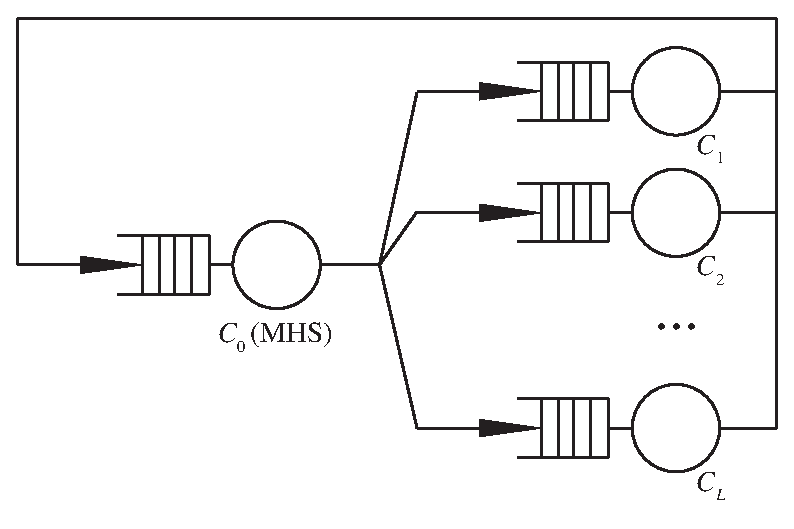
\includegraphics[]{FMS}
  \caption{Схема гибкой производственной системы}
  \label{fig:fms}
\end{figure}

Функционирование гибкой производственной системы происходит следующим образом.

Система должна обработать $t=1,2,...,T$ типов деталей. Общее число деталей в системе в любой момент времени постоянно и равно $N$. Другими словами, все доступные палеты все время заняты. Всякий раз, когда обработанная деталь покидает систему, другая деталь того же типа сразу же поступает в систему. Это неявно предполагает, что имеется непрерывное снабжение системы деталями для их обработки. Далее будет рассматриваться только долгосрочное поведение гибкой производственной системы или стационарный режим функционирования. Число палет $N_t$, выделяемых для деталей типа $t$, постоянно и $\sum\limits_t N_t = N$. Определим вектор начального числа деталей $\mathbf{N}=(N_t)$, $t=1,...,T$.

Рабочие станции или машины могут быть свободны (простаивать), но они никогда не блокируются. На практике это, как правило, обеспечивается за счет \textit{возвратного конвейера}, который постоянно забирает из рабочих станций детали, завершившие обработку, и доставляет их обратно в центральное хранилище (предполагается, что в центральном хранилище достаточно мест для размещения всех деталей в случае необходимости, т.е. $s_0=N$). Задержка деталей на возвратном конвейере не учитывается. В этом смысле емкость хранилища возвратного конвейера является частью емкости центрального хранилища.

Деталь каждого типа $t$ нуждается во множестве операций, которые будут выполняться на наборе рабочих станций с номерами $I_t \subseteq I$. Длительность обработки детали типа $t$ на станции $C_i$, $i \in I_t$, имеет экспоненциальное распределение с параметром $\mu_{it}$. Пусть $s_{it}$~--- емкость места хранения, выделенного для деталей типа $t$ на станции $C_i$. Пусть $s_{it}=0$, если $i \notin I_t$, тогда $\sum\limits_t s_{it} = s_i$.

Длительность обработки детали на станции $C_0$ включает в себя время перехода детали на следующую станцию, а также время для погрузки/разгрузки и повторной установки в случае необходимости. Распределение длительности обработки деталей типа $t$ также предполагается экспоненциальным с параметром $\mu_{0t}$.

Дисциплина обработки на всех станциях $C_i,~i=0,...,L$,~--- \textit{RANDOM} (то есть детали выбираются для обработки случайным образом). Для определенности предполагается, что для каждой станции $C_i$ среднее число приборов (механизмов/транспортеров), обрабатывающих детали типа $t$, пропорционально $n_{it}$~--- количеству деталей типа $t$ на станции $C_i$. Определим вектор размерности $Т$
\begin{equation*}
 \overline{\eta}_i = (n_{i1},...,n_{iT}), \quad \text{где}~ n_{it}=0, ~\text{если}~ i \notin I_t, ~\text{и пусть}~ n_i = \sum_{t=1}^{T} n_{it}.
\end{equation*}
Вектор $\overline{\eta}_i$ определяет состояние станции $C_i$ как вектор числа деталей различных типов, находящихся на этой станции.
Суммарная интенсивность обработки деталей типа $t$ на станции $C_i$ может быть выражена в виде
\begin{equation*}
 \mu_{it} n_{it} \nu_{i}(n_i), \quad \text{где} ~\nu_i(n_i) = \frac{\min(n_i, \kappa_i)}{n_i}.
\end{equation*}

На станции $C_0$ решения, связанные с маршрутизацией, принимаются всякий раз, когда транспортер становится доступным. Согласно описанной выше дисциплине обслуживания \textit{RANDOM}, если деталь типа $t$ должна быть доставлена следующей, то для доставки выбирается некоторая станция с номером $i \in I_t$, которая имеет наибольшее число свободных мест, т.е. $s_{it} - n_{it} \geqslant s_{kt} - n_{kt}$ для всех $k \in I_t$ и $k \neq i$. Одна из деталей типа $t$, ожидающая в центральном хранилище обработки на станции $C_i$ (эту деталь будем называть <<очередной>> деталью), затем доставляется на станцию $C_i$. Эта схема маршрутизации называется детерминированной маршрутизацией в кратчайшую очередь или DSQ--маршрутизацией.

Пусть $\Theta = (\theta_{it,jt})$~--- маршрутная матрица, $t=1,...,T$, $i,j=0,...,L$, где $\theta_{it,jt}$~--- вероятность того, что деталь типа $t$ после обработки на станции $C_i$ поступает на станцию $C_j$. Заметим, что допускаются переходы только из системы транспортировки на рабочие станции и из рабочих станций в систему транспортировки, т.е. $\theta_{it,jt}=0$ при $i,j>0$. Также заметим, что деталь типа $t$ может перемещаться только на рабочую станцию из множества $I_t \subseteq I$, то есть $\theta_{it,jt'}=0$ при $t \neq t'$.

\textbf{Примечания}

\begin{enumerate}
\item Назначение палет и емкости хранилища для различных типов деталей (например, $N_t$ и $s_{it}$) будет непосредственно влиять на маршрутизацию и, следовательно, пропускную способность для каждого типа деталей. Выбор этих параметров должен быть согласован с желаемой пропускной способностью типов деталей.

\item Две главных цели гибких производственных систем состоят в том, чтобы уменьшить в хранилище число необработанных деталей и увеличить коэффициент использования приборов на станциях. Известно, что с использованием приборов главным образом связаны два фактора: блокирование и простаивание (здесь не рассматриваются проблемы надежности). Ранее сделанные предположения о возвратном конвейере и центральном хранилище позволяют увеличить коэффициент использования приборов за счет исключения возможности их блокирования. С другой стороны, также известно, что простаивание прибора в первую очередь влияет на интенсивность потока и загрузку каждой станции. Локальные буферы могут уменьшить влияние простаивания прибора, но, конечно, не в значительной мере. Тогда, в целях сокращения в хранилище числа необработанных деталей, предполагается наличие ограниченных локальных буферов на станциях. Исследования существующих гибких производственных систем показывают, что большинство из них имеют очень маленькие локальные буферы. Некоторые производственные системы, которые используют замкнутые конвейеры в качестве системы транспортировки материалов, имеют нулевые локальные буферы: ожидающие детали просто стоят на конвейере, который функционирует и как устройство транспортировки материалов, и как центральное хранилище.

\item В рассматриваемой в данной работе модели маршрутизация деталей определяется для \textit{потока} деталей в рабочую станцию (на обрабатывающие приборы), а не для \textit{отдельных} деталей. Всякий раз, когда решение, связанное с маршрутизацией, должно быть принято, сначала определяется соответствующая рабочая станция (прежде всего те, которые содержат наименьшее число деталей), а затем некоторая деталь <<вытаскивается>> из центрального хранилища для доставки на эту станцию.
\end{enumerate}

Данная гибкая производственная система с введенными выше предположениями описывается неоднородной замкнутой экспоненциальной сетью массового обслуживания $\Gamma=\left<L,T,\mathbf{N},N,M,\Theta,\kappa,\mu,\textit{RANDOM}\right>$. В дальнейшем термины <<гибкая производственная система>>, <<рабочая станция>>, <<обрабатывающий прибор>>, <<детали>>, <<обработка деталей>>, использующиеся для описания гибких производственных систем, будем отождествлять соответственно с терминами <<сеть массового обслуживания>>, <<система>>, <<обслуживающий прибор>>, <<требования>>, <<обслуживание требований>>.

\subsection{Решение уравнения равновесия}
\label{subsec:solution}

Определим состояние сети $\Gamma$, соответствующей рассмотренной выше гибкой производственной системе, как $\overline{\eta} = (\overline{\eta}_0, \overline{\eta}_1,...,\overline{\eta}_L)$, где $\overline{\eta}_i = (n_{i1},...,n_{iT})$, $i=0,1,...,L$, обозначает вектор числа требований в системе $C_i$. Из предположений в разделе~\ref{subsec:FMS_specification} нетрудно видеть, что $\{ \overline{\eta}(\tau) \}$ определяет процесс Маркова со следующим конечным пространством состояний:
\begin{equation}
 S = \left\lbrace \overline{\eta} \in Z_+^{(L+1)T} ~|~ n_{it} \leqslant s_{it} ~ (i \in I), ~
 \sum_{i \in I_t^+} n_{it} = N_{t}, ~ t=1,...,T \right\rbrace ,
 \label{eq:2.1}
\end{equation}
где $Z_+$ обозначает множество неотрицательных чисел и $I_t^+ = \{ 0 \} \cup I_t$.

В дальнейшем внесем элемент случайности в детерминированную маршрутизацию в кратчайшую очередь (DSQ--маршрутизацию), при которой требования направляются в кратчайшую очередь с наибольшей вероятностью (с вероятностью один), с помощью PSQ--маршрутизации. Установлено, что PSQ--маршрутизация~--- точное приближение DSQ--маршрутизации при условии, что емкости систем намного меньше общего числа требований в сети $N$ (которое, как правило, справедливо для реальных производственных систем) \cite{yao1}.

Сформулируем PSQ--маршрутизацию следующим образом. Вероятности перехода требований класса $t$ из системы $C_0$ в систему $C_i$, $i \in I_t$, зависят от $n_{0t}$ и от $n_{it}$~--- числа требований класса $t$ в двух системах, и принимают форму
\begin{equation}
 \theta_{0t,it} = \frac{r_{it}(n_{it})} {r_{0t}(n_{0t})},
\label{eq:2.2}
\end{equation}
где $r_{it}(\cdot)$ и $r_{0t}(\cdot)$~--- две линейные функции:
\begin{equation*}
 r_{it}(n_{it}) = s_{it} - n_{it} ~ \text{и} ~ r_{0t}(n_{0t}) = \sum_{C_i \in I_t} s_{it} + n_{0t} - N_t .
\end{equation*}
Заметим, что $r_{it}(\cdot)$ показывают число свободных мест в системе $C_i$ для требований класса $t$, а $r_{0t}(n_{0t}) = \sum\limits_{C_i \in I_t} r_{it}(n_{it})$ такие, что маршрутные вероятности в сумме по всем $i \in I_t$ равны единице. Несложно заметить следующие особенности этой схемы маршрутизации:
\begin{itemize}
\item маршрутные вероятности выше для систем с б\'{о}льшим числом свободных приборов;
\item требования класса $t$ никогда (т.е. с вероятностью ноль) не направляются в систему, в которой все места в очереди для ожидания требованиями этого класса заняты (т.е. когда $n_{it} = s_{it}$).
\end{itemize}

Для того, чтобы получить решение для сети $\Gamma$ как модели гибкой производственной системы, понадобятся следующие предварительные сведения об обратимых марковских процессах.

\begin{definition}
 Случайный процесс $\{ X(\tau) \}$ (время $\tau \in T$ может быть непрерывным или дискретным), определенный в пространстве состояний $S$ (конечном или счетном), является обратимым, если $\{ X(\tau_1),...,X(\tau_n) \}$ имеет то же распределение, что и $\{ X(\tau_0 - \tau_1),...,X(\tau_0 - \tau_n) \}$ для всех $\tau_0, \tau_1,..., \tau_n \in T$~\cite{kelly}.
\end{definition}

Обратимый процесс, как известно, является стационарным. Для стационарных марковских процессов имеет место следующее утверждение.

\begin{lemma}
 Стационарный марковский процесс $\{ X(\tau) \}$ является обратимым, если существует положительный набор чисел $\pi(j), j \in S$, в сумме дающий единицу, который удовлетворяет следующим уравнениям равновесия:
 \begin{equation}
  \pi(j) q(j,k) = \pi(k) q(k,j) \quad \forall j,k \in S ,
  \label{eq:2.3}
 \end{equation}
 где $q(j,k)$~--- интенсивность перехода из состояния $j$ в состояние $k$. Если существует такой набор $\pi(j), j \in S$, то он является стационарным распределением процесса $X(\tau)$~\cite{kelly}.
\end{lemma}

Стационарное решение для сети $\Gamma$ как модели гибкой производственной системы можно теперь обобщить следующим образом.

\begin{theorem}
 Марковский процесс $\overline{\eta}(\tau)$, определенный в пространстве состояний $S$ и управляемый PSQ--маршрутизацией, как определено в~(\ref{eq:2.2}), является обратимым относительно времени и имеет следующую мультипликативную форму стационарного распределения вероятностей:
 \begin{equation}
  \pi(\overline{\eta}) = G^{-1} \prod_{i=0}^L \left[ \prod_{j=1}^{n_i} \nu_i^{-1} (j) \right]
  \left[ \prod_{t=1}^T \prod_{j=1}^{n_{it}} \frac{r_{it} (j - 1 + \delta_{i0})}{j\mu_{it}} \right], \quad \overline{\eta} \in S ,
  \label{eq:2.4}
 \end{equation}
где $\delta_{i0}=1$, если $i=0$, иначе $\delta_{i0}=0$, и $G$~--- нормализующая константа.
\end{theorem}

\begin{proof}
 Пусть вектор $\overline{\eta}'$ обозначает состояние сети $\Gamma$ c компонентами
  \begin{equation*}
   \overline{\eta}_0 ' = (n_{01},...,n_{0u}-1,...,n_{0T}), \quad \overline{\eta}_k ' = (n_{k1},...,n_{ku}+1,...,n_{kT}),
  \end{equation*}
 а все остальные компоненты такие же как у вектора $\overline{\eta}$ (т.е. требование класса $u$ перешло из системы $C_0$ в систему $C_k$). Основываясь на лемме, достаточно показать, что определенное в~(\ref{eq:2.4}) распределение $\pi(\overline{\eta})$ (для всех $\overline{\eta} \in S$) удовлетворяет следующим уравнениям равновесия: для $\overline{\eta}, \overline{\eta} ' \in S$
 \begin{equation}
  \pi(\overline{\eta}) [n_{0u} \mu_{0u} \nu_0(n_0)] \left[ \frac{r_{ku} (n_{ku})}{r_{0u} (n_{0u}) } \right]  =
  \pi(\overline{\eta} ') [(n_{ku} + 1)\mu_{ku} \nu_k (n_k + 1)] ,
  \label{eq:2.5}
 \end{equation}
 где величины в квадратных скобках левой части дают вероятность перехода сети из состояния $\overline{\eta}$ в состояние $\overline{\eta} '$, а величины в квадратных скобках правой части дают вероятность перехода сети из состояния $\overline{\eta} '$ в состояние $\overline{\eta}$. Выражение~(\ref{eq:2.5}) эквивалентно следующему:
 \begin{equation*}
  \pi(\overline{\eta} ') \left[ \frac{r_{0u} (n_{0u})}{n_{0u} \mu_{0u} \nu_0(n_0)} \right]
  \left[ \frac{(n_{ku} + 1)\mu_{ku} \nu_k (n_k + 1)}{r_{ku} (n_{ku})} \right] = \pi(\overline{\eta}) .
  \tag{\theequation a} \label{eq:2.5a}
 \end{equation*}
 Из (\ref{eq:2.4}) запишем $\pi(\overline{\eta})$ как
 \begin{equation*}
  \pi(\overline{\eta}) = G^{-1} \prod_{i=0}^L F_i(\overline{\eta}_i) ,
 \end{equation*}
 где $F_i(\overline{\eta}_i)$ обозначают величины в двух квадратных скобках правой части выражения~(\ref{eq:2.4}). Тогда $\pi(\overline{\eta}')$ может быть соответственно выражено следующим образом:
 \begin{equation*}
  \pi(\overline{\eta} ') = G^{-1} \prod_{i \neq 0,k} F_i(\overline{\eta}_i)
  [F_0(\overline{\eta}_0 ')F_k(\overline{\eta}_k ')] ,
 \end{equation*}
 где
 \begin{equation*}
  F_0(\overline{\eta}_0 ') = \prod_{j=1}^{n_0-1} \nu_0^{-1}(j) \cdot
  \left[
  \prod_{t \neq u} \prod_{j=1}^{n_{0t}} \frac{r_{0t}(j)}{j\mu_{0t}} \cdot,
  \prod_{j=1}^{n_{0u}-1} \frac{r_{0u}(j)}{j\mu_{0u}}
  \right] ,
 \end{equation*}

 \begin{equation*}
  F_k(\overline{\eta}_k ') = \prod_{j=1}^{n_k+1} \nu_k^{-1}(j) \cdot
  \left[
  \prod_{t \neq u} \prod_{j=1}^{n_{kt}} \frac{r_{kt}(j-1)}{j\mu_{kt}} \cdot
  \prod_{j=1}^{n_{ku}+1} \frac{r_{ku}(j-1)}{j\mu_{ku}}
  \right] .
 \end{equation*}
 Тогда очевидно, что
 \begin{equation*}
  F_0(\overline{\eta}_0 ') \cdot \left[ \frac{r_{0u}(n_{0u})}{n_{0u}\mu_{0u}\nu_0(n_0)} \right] =
  F_0(\overline{\eta}_0)
 \end{equation*}

 \begin{equation*}
  F_k(\overline{\eta}_k ') \cdot \left[ \frac{(n_{ku}+1) \mu_{ku} \nu_k (n_k+1)}{r_{ku}(n_{ku})} \right] =
  F_k(\overline{\eta}_k)
 \end{equation*}
 и, следовательно, равенство (\ref{eq:2.5a}) верно. Таким образом, теорема доказана.
\end{proof}


%%%%%%%%%%%%%%%%%%%%%%%%%%%%%%%%%%%%%%%%%%%%%%%%%%%%%%%%%%%%%%%%%%%%%%%%%%%%%%%


\section{Алгоритм метода анализа производственных систем с~маршрутизацией, зависящей от состояния}
\label{sec:algorithm}

\subsection{Описание алгоритма}
\label{subsec:algorithm_description}

Рассмотрим однородную замкнутую экспоненциальную сеть массового обслуживания $\Gamma'~=~\langle L, 1, N, M, \Theta, \kappa, \mu, FCFS \rangle$ с $L$ системами $C_i$, $i=1,...,L$, (включая систему транспортировки материалов, которая теперь обозначается как любая $C_i$) и $N$ требованиями (палетами в ГПС). Сначала рассмотрим случай одного класса требований ($T=1$). Обобщение на случай нескольких классов требований рассматривается в конце раздела.

При $Т=1$ будем опускать индекс $t$, выразим $\pi(\overline{\eta})$ следующим образом:
\begin{equation}
 \pi(\overline{\eta}) = G^{-1}(L,N) \prod_{i=1}^L F_i(n_i) = G^{-1}(L,N) \prod_{i=1}^L
 \prod_{j=1}^{n_{i}} f_i(j) ,
 \label{eq:3.1}
\end{equation}
где $G(L,N)$~--- нормализующая константа, а $f_i(\cdot)$~--- множитель $F_i(\cdot)$, равный
\begin{equation*}
f_i(j) = \nu_i^{-1}(j) \frac{r_i(j-1+\delta_{i0})}{j \mu_i}.
\end{equation*}
При $T=1$ дисциплина обслуживания эквивалентна дисциплине <<первым пришел ~--- первый обслужен>> (FCFS).

Кроме того, обозначим через $G(L-1,N)$ нормализующую константу, связанную с сетью из $L-1$ системы, где $L$--ая система удалена. Пусть
\begin{equation*}
R(L,N) = \frac{G(L,N-1)}{G(L,N)}
\end{equation*}
и определим аналогичным образом $R(L-1,N)$.

Не теряя общности, предположим, что требуется получить предельное маргинальное (частное) распределение вероятностей $\pi_L(k,N)~(k=0,1,...,s_L)$ для системы $C_L$ сети $\Gamma'$ с $L$ системами и $N$ требованиями. Имеют место следующие рекуррентные формулы.

\begin{proposition}
 \begin{equation}
  \pi_L(0,N) = \pi_L(0,N-1) R^{-1}(L-1,N) R(L,N) ,
  \label{eq:3.2}
 \end{equation}
 \begin{equation}
  \pi_L(k,N) = \pi_L(k-1,N-1) f_L(k) R(L,N) \quad (k=1,2,...,s_L) .
  \label{eq:3.3}
 \end{equation}
\end{proposition}

\begin{proof}
 Из (\ref{eq:3.1}) и обозначений, определенных выше, имеем
 \begin{multline*}
  \pi_L(0,N) = \frac{G(L-1,N)}{G(L,N)} = \frac{G(L-1,N-1)}{G(L,N-1)} \cdot \frac{G(L-1,N)}{G(L-1,N-1)} \cdot
  \frac{G(L,N-1)}{G(L,N)} = \\ \\
  = \pi_L(0,N-1) R^{-1}(L-1,N) R(L,N) .
 \end{multline*}
 Для $k=1,2,...,s_L$ имеем
  \begin{multline*}
  \pi_L(k,N) = F_L(k) \cdot \frac{G(L-1,N-k)}{G(L,N)} = \\ \\
  = f_L(k) F_L(k-1) \cdot \frac{G(L-1,N-1-(k-1))}{G(L,N-1)} \cdot \frac{G(L,N-1)}{G(L,N)} = \\ \\
  = \pi_L(k-1,N-1) f_L(k) R(L,N) .
 \end{multline*}
\end{proof}

На основе приведенных выше результатов разработан алгоритм, аналогичный алгоритму нормализованной свертки Райзера~\cite{reiser}, который предназначен в основном для замкнутых сетей с постоянной маршрутизацией требований и неограниченными очередями в системах сети.

Предположим, что мы хотим проанализировать сеть с $N$ требованиями и $L$ системами. Для рекурсивного вычисления $R(L,N)$ и $\pi_L$ имеется три цикла: \\
цикл I по числу систем от $m=1$ до $m=L$; \\
цикл II для каждого $m$ по числу требований от $n=0$ до $n~=~\min(N, \sum\limits_{i=1}^m s_i)$; \\
цикл III для каждого $n$ по общему числу требований в системе $C_m$ от $k=0$ до $k=\min(s_m,n)$.

Заметим, что II и III цикл здесь отличаются от циклов в алгоритме свертки Райзера. Пределы здесь также ограничены: $R(1,n) = f_1^{-1}(n), n=1,...,s_1$. Как и в алгоритме свертки Райзера, при расчете значений $\pi_m$ итоговая константа $R(m,n)$ сначала может не учитываться, а затем может быть рассчитана как нормирующий множитель:
\begin{equation*}
 R(m,n) = \left[ \sum_{k=0}^{s_m} \pi_m(k,n) \right] ^ {-1} \quad \text{(}
 \pi_m \text{-ые в сумме ненормированные)} .
\end{equation*}
Таким образом, $R(L,n)$ и $\pi_L$--ые по-прежнему могут быть получены одновременно. После нахождения $R(L,n)~(n=1,...,N)$ сразу получаем
\begin{equation}
 G(L,N) = \prod_{n=1}^N R^{-1}(L,n) .
 \label{eq:9}
\end{equation}

Алгоритм анализа однородной сети следующий:

\begin{tabbing}
\textit{Шаг 0.} \= (Инициализация) \\
\> $m = 1$ \\
\> $\textit{NN}_{1} = s_{1}$ \\
\>  Для $n=1$ до $\textit{NN}_{1}$: $R(n) = f_{1}^{-1}(n)$: следующее $n$. \\
\textit{Шаг 1.} \= (Цикл I) \\
\> $m = m + 1$ \\
\> $\textit{NN}_{m} = \min(N, N_{m-1} + s_{m})$ \\
\> $\pi(0) = 1$ \\
\textit{Шаг 2.} \= (Цикл II) \\
\> Для $n=1$ до $\textit{NN}_{m}$ \\
\> \quad $\text{sum} = 0$ \\
\> \quad $kk = \min(s_{m},n)$ \\
\> \quad (Цикл III) \\
\> \quad Для $k = kk$ до $1$ \\
\> \quad \quad $\pi(k) = \pi(k-1) * f_{m}(k)$ \\
\> \quad \quad $\text{sum} = \text{sum} + \pi(k)$ \\
\> \quad следующее $k$. \\
\> \quad Если $n > \textit{NN}_{m-1}$, то $\pi(0) = 0$, иначе $\pi(0) = \pi(0)/R(n)$ \\
\> \quad $R(n) = 1 / [\text{sum} + \pi(0)]$ \\
\> \quad Для $k = 0$ до $kk$: $\pi(k) = \pi(k) * R(n)$: следующее $k$ \\
\> следующее $n$. \\
\textit{Шаг 3.} \= Если $m < L$ то перейти на \textit{шаг 1} \\
\> иначе вернуть результат. Останов.
\end{tabbing}

Как и в алгоритме нормализованной свертки Райзера, алгоритм использует два одномерных массива: $R(n)$ (размерности $N+1$) и $\pi(k)$ (размерности $\max\limits_{i} s_i+1$).

В общем случае, для сети массового обслуживания с несколькими классами требований определим векторы размерности $T$: $\mathbf{N}=(N_1,...,N_T)$, $\mathbf{n}=(n_1,...,n_T)$, $\mathbf{e_t}=(0,...,1,...,0)$ ($t$--ый элемент равен $1$, а все остальные нули) и $\mathbf{0}=(0,...,0)$. Пусть $G(m,\mathbf{N})$ будет нормализующей константой, где $\mathbf{N}$~--- вектор начального числа требований в сети. Кроме того, определим
\begin{equation*}
R_t(m,\mathbf{N}) = \frac{G(m,\mathbf{N}-\mathbf{e_t})}{G(m,\mathbf{N})},~~t=1,...,T.
\end{equation*}
Обозначим через $\pi_m(\mathbf{n},\mathbf{N})$ предельную вероятность того, что общее число требований в системе $m$ будет равно $\mathbf{n}$, когда общее число требований всей сети равно $\mathbf{N}$. Тогда справедливо следующее следствие.

\begin{corollary}
 Если $\mathbf{n} > \mathbf{0}$ (т.е. все элементы вектора $\mathbf{n}$ положительны), то для всех $t=1,...,T$
 \begin{equation}
  \pi_m(\mathbf{n},\mathbf{N}) = \pi_m(\mathbf{n}-\mathbf{e_t},\mathbf{N}-\mathbf{e_t})
  f_{mt}(\mathbf{n}) R_t(m,\mathbf{N}) ,
  \label{eq:10}
 \end{equation}
 иначе для всех $t=1,...,T$
  \begin{equation}
  \pi_m(\mathbf{n},\mathbf{N}) = \pi_m(\mathbf{n},\mathbf{N}-\mathbf{e_t}) R_t^{-1}(m-1,\mathbf{N}-\mathbf{n}) R_t(m,\mathbf{N}) .
  \label{eq:11}
 \end{equation}
\end{corollary}

Разработанный ранее алгоритм применим и здесь со следующими изменениями.
\begin{enumerate}
\item Необходимы два двухмерных массива для $\pi(\mathbf{n})$ и $R_t$, $t=1,...,T$.
\item В этом случае имеется $T$ нормализующих множителей $R_t$, $t=1,...,T$, которые в дополнение к условию нормировки значений $\pi_m$ удовлетворяют следующим уравнениям:
\begin{equation}
 R_t(m,\mathbf{N}) = R_t(m-1,\mathbf{N}) \frac{\pi_m(\mathbf{0},\mathbf{N})}
 {\pi_m(\mathbf{0},\mathbf{N}-\mathbf{e_t})}, \quad t=1,...,T .
 \label{eq:12}
\end{equation}
Эти уравнения следуют непосредственно из~(\ref{eq:11}) при предположении, что $\mathbf{n}=\mathbf{0}$.
\end{enumerate}

Алгоритм для неоднородной сети приведен в следующем разделе.


\subsection{Структурная схема алгоритма}
\label{subsec:flowchart}

Алгоритм метода анализа сети массового обслуживания $\Gamma$ с маршрутизацией, зависящей от состояния, имеет блочную структуру, представленную на рисунке \ref{img:4.1}.

\begin{figure}[H]
\centering
\tikzstyle{arrow} = [draw, ->, >=angle 60]
\tikzstyle{block} = [rectangle, draw, text width=16em, text centered]
\tikzstyle{inout} = [trapezium, draw, text width=10em, text centered, trapezium left angle=70,trapezium right angle=-70]
\tikzstyle{for} = [shape=chamfered rectangle, chamfered rectangle xsep=2cm, draw]
\begin{tikzpicture}[node distance = 2cm, auto]
\node [rounded rectangle, draw] (begin) {Начало};
\node [inout, below of=begin] (init) {Блок 1. Ввод исходных данных};
\node [for, below of=init] (for) {$i=1,2,...,L$};
\node [block, below of=for] (renum) {Блок 2. Перестановка СМО $C_i$ и $C_L$};
\node [block, below of=renum, node distance = 2.5cm] (pi) {Блок 3. Вычисление стационарного распределения вероятностей СМО $C_i$};
\node [block, below of=pi, node distance = 2.5cm] (renum_back) {Блок 4. Обратная перестановка СМО $C_L$ и $C_i$};
\node [block, below of=renum_back, node distance = 4.5cm] (parameters) {Блок 5. Вычисление стационарных характеристик СеМО};
\node [inout, below of=parameters, node distance = 2.5cm] (output) {Блок 6. Вывод результатов};
\node [rounded rectangle, draw, below of=output] (end) {Конец};
\path [arrow] (begin) -- (init);
\path [arrow] (init) -- (for);
\path [arrow] (for) -- (renum);
\path [arrow] (renum) -- (pi);
\path [arrow] (pi) -- (renum_back);
\path [arrow] (renum_back) -- ++(0,-2) -- ++(-6,0) |- (for);
\path [arrow] (for) -- ++(6,0) -- ++(0,-10) -| (parameters);
\path [arrow] (parameters) -- (output);
\path [arrow] (output) -- (end);
\end{tikzpicture}
\caption{Блок-схема алгоритма метода анализа сетей массового обслуживания с маршрутизацией, зависящей от состояния}
\label{img:4.1}
\end{figure}

\medskip
\textbf{Блок 1. Ввод исходных данных}

На начальном этапе работы алгоритма вводятся параметры сети массового обслуживания $\Gamma$:\\
$L$~--- число СМО в СеМО;\\
$\mathbf{N}=(N_t)$~--- вектор начального числа требований в СеМО, $t=1,...,T$;\\
$\kappa=(\kappa_i)$~--- вектор числа приборов в системах обслуживания СеМО, $i=0,...,L$;\\
$s=(s_{it})$~--- матрица емкостей систем в СеМО, $i=0,...,L,~t=1,...,T$;\\
$\mu=(\mu_{it})$~--- матрица интенсивностей обслуживания требований системами СеМО, $i=0,...,L,~t=1,...,T$.

\medskip
\textbf{Блок 2. Перестановка СМО $\boldsymbol{C_i}$ и $\boldsymbol{C_L}$}

Во втором блоке для вычисления стационарного распределения вероятностей состояний системы $C_i,~i=1,...,L,$ происходит перестановка системы $C_i$ с последней системой $C_L$. Это осуществляется путем перестановки элементов $\kappa_i$ и $\kappa_L$ в векторе $\kappa$, $s_{it}$ и $s_{iL}$ в матрице $s$, $\mu_{it}$ и $\mu_{iL}$ в матрице $\mu$, $i=1,...,L,~t=1,...,T$. \\
\textit{Входные данные:} $\kappa=(0,...,\kappa_i,...,\kappa_L)$, $s=\left( \begin{matrix}
s_{1t}\\
\cdots\\
s_{it}\\
\cdots\\
s_{Lt}
\end{matrix} \right )$, $\mu=\left( \begin{matrix}
\mu_{1t}\\
\cdots\\
\mu_{it}\\
\cdots\\
\mu_{Lt}
\end{matrix} \right )$, $t~=~1,...,T$. \\
\textit{Выходные данные:} $\kappa'=(0,...,\kappa_L,...,\kappa_i)$, $s'=\left( \begin{matrix}
s_{1t}\\
\cdots\\
s_{Lt}\\
\cdots\\
s_{it}
\end{matrix} \right )$, $\mu'=\left( \begin{matrix}
\mu_{1t}\\
\cdots\\
\mu_{Lt}\\
\cdots\\
\mu_{it}
\end{matrix} \right )$, $t=1,...,T$.

\medskip
\textbf{Блок 3. Вычисление стационарного распределения вероятностей состояний СМО $\boldsymbol{C_i}$}

Алгоритм для вычисления стационарного распределения вероятностей состояний для системы $C_i$ следующий:\\
\emph{Входные данные:} $L$, $T$, $\mathbf{N}=(N_t)$, $\kappa=(\kappa_i)$, $s=(s_{it})$, $\mu=(\mu_{it})$, $i=0,...,L,~t=1,...,T$.

\begin{tabbing}
\textit{Шаг 0.} \= \\
\> $t = 0$ \\
\> $m = 0$ \\
\textit{Шаг 1.} \= (Цикл I) \\
\> $t = t + 1$ \\
\> $\textit{NN}_{t0} = s_{0t}$ \\
\>  Для $n=1$ до $\textit{NN}_{t0}$: $R_t(n) = f_{t0}^{-1}(n)$: следующее $n$. \\
\textit{Шаг 2.} \= (Цикл II) \\
\> $m = m + 1$ \\
\> $\textit{NN}_{tm} = \min(N_t, N_{t,m-1} + s_{mt})$ \\
\> $\pi_i(0,N_t) = 1$ \\
\textit{Шаг 3.} \= (Цикл III) \\
\> Для $n=1$ до $\textit{NN}_{tm}$ \\
\> \quad $\text{sum} = 0$ \\
\> \quad $kk = \min(s_{mt},n)$ \\
\> \quad (Цикл IV) \\
\> \quad Для $k = kk$ до $1$ \\
\> \quad \quad $\pi_i(k,N_t) = \pi_i(k-1,N_t) * f_{tm}(k)$ \\
\> \quad \quad $\text{sum} = \text{sum} + \pi_i(k,N_t)$ \\
\> \quad следующее $k$. \\
\> \quad Если $n > \textit{NN}_{t,m-1}$, то $\pi_i(0,N_t) = 0$, иначе $\pi_i(0,N_t) = \pi_i(0,N_t)/R_t(n)$ \\
\> \quad $R_t(n) = 1 / [\text{sum} + \pi_i(0,N_t)]$ \\
\> \quad Для $k = 0$ до $kk$: $\pi_i(k,N_t) = \pi_i(k,N_t) * R_t(n)$: следующее $k$ \\
\> следующее $n$. \\
\textit{Шаг 4.} \= Если $m < L$ то перейти на \textit{шаг 3} \\
\textit{Шаг 5.} \= Если $t < T$ то перейти на \textit{шаг 2} \\
\> иначе вернуть результат. Останов.
\end{tabbing}
Функция $f_{tm}(k)$ в алгоритме определяется как
\begin{equation*}
f_{tm}(k) = \nu_m^{-1}(k) \frac{r_{it}(k-1+\delta_{m0})}{k \mu_{mt}}.
\end{equation*}
\emph{Выходные данные:} $\pi_i(\mathbf{n},\mathbf{N})$, $i=1,...,L$.

\medskip
\textbf{Блок 4. Обратная перестановка СМО $\boldsymbol{C_L}$ и $\boldsymbol{C_i}$}

Происходит обратная перестановка системы $C_ L$ с системой $C_i$. Таким образом, получаем исходный вектор $\kappa$ и матрицы $s$, $\mu$. \\
\textit{Входные данные:} $\kappa'=(0,...,\kappa_L,...,\kappa_i)$, $s'=\left( \begin{matrix}
s_{1t}\\
\cdots\\
s_{Lt}\\
\cdots\\
s_{it}
\end{matrix} \right )$, $\mu'=\left( \begin{matrix}
\mu_{1t}\\
\cdots\\
\mu_{Lt}\\
\cdots\\
\mu_{it}
\end{matrix} \right )$, $t=1,...,T$. \\
\textit{Выходные данные:} $\kappa=(0,...,\kappa_i,...,\kappa_L)$, $s=\left( \begin{matrix}
s_{1t}\\
\cdots\\
s_{it}\\
\cdots\\
s_{Lt}
\end{matrix} \right )$, $\mu=\left( \begin{matrix}
\mu_{1t}\\
\cdots\\
\mu_{it}\\
\cdots\\
\mu_{Lt}
\end{matrix} \right )$, $t~=~1,...,T$.

\medskip
\textbf{Блок 5. Вычисление стационарных характеристик СеМО}

На данном этапе происходит вычисление следующих стационарных характеристик СеМО:
\begin{itemize}
\item м. о. числа $t$-требований в СМО;
\item м. о. числа занятых $t$-требованиями приборов в СМО;
\item интенсивность входящего потока $t$-требований в СМО;
\item коэффициенты использования обслуживающих приборов СМО $t$~-~требованиями.
\end{itemize}
Эти характеристики вычисляются по формулам (\ref{eq:distribution_n}) -- (\ref{eq:distribution_psi0}).\\
\begin{equation}
\overline{n}_{it} = \sum\limits_{k=0}^{s_{it}} k \pi_i(\mathbf{n},\mathbf{N}),
 \label{eq:distribution_n}
\end{equation}
\begin{equation}
\overline{h}_{it} = \left\{
 \begin{array}{l}
 \sum\limits_{k=0}^{\kappa_i} k \pi_i(\mathbf{n},\mathbf{N}) + \kappa_i  \sum\limits_{k=\kappa_i + 1}^{s_{it}} \pi_i(\mathbf{n},\mathbf{N}), \quad \kappa_i < s_{it}, \\
 \sum\limits_{k=0}^{s_{it}} k \pi_i(\mathbf{n},\mathbf{N}), \quad \kappa_i \ge s_{it},
 \end{array}
\right.
 \label{eq:distribution_h}
\end{equation}
\begin{equation}
\lambda_{it} = \mu_{it} \overline{h}_{it},
 \label{eq:distribution_lambda}
\end{equation}
\begin{equation}
\psi_{it} = \frac{\lambda_{it}}{\min(\kappa_{i}, s_{it}) \mu_{it}},
 \label{eq:distribution_psi}
\end{equation}
где $i=1,...,L,~t=1,...,T$.
\begin{equation}
\overline{n}_{0t} = N_t - \sum\limits_{i=1}^L \overline{n}_{it},
 \label{eq:distribution_n0}
\end{equation}
\begin{equation}
\lambda_{0t} = \sum\limits_{i=1}^L \lambda_{it},
 \label{eq:distribution_lambda0}
\end{equation}
\begin{equation}
\psi_{0t} = \frac{\lambda_{0t}}{\kappa_0 \mu_{0t}},
 \label{eq:distribution_psi0}
\end{equation}
где $t=1,...,T$. \\
\emph{Входные данные:} $L$, $T$, $\mathbf{N}=(N_t)$, $\pi_m(\mathbf{n},\mathbf{N})$, $\kappa=(\kappa_i)$, $s=(s_{it})$, $\mu=(\mu_{it})$, $i=0,...,L,~m=1,...,L,~t=1,...,T$.\\
\emph{Выходные данные:} $\overline{n}_{it}$, $\lambda_{it}$, $\psi_{it}$, $i=0,...,L,~t=1,...,T$.

\medskip
\textbf{Блок 6. Вывод результатов}

В данном блоке происходит вывод (на экран или в файл) стационарного распределения и стационарных характеристик, полученных в блоке 4 и 5.\\


%%%%%%%%%%%%%%%%%%%%%%%%%%%%%%%%%%%%%%%%%%%%%%%%%%%%%%%%%%%%%%%%%%%%%%%%%%%%%%%


\section{Описание и назначение программы}
\label{sec:program_description_and_purpose}

Программа, предназначенная для  анализа производственных систем с маршрутизацией, зависящей от состояния, была реализована на языке программирования Java на платформе JDK 7 с использованием стандартной библиотеки для создания графического интерфейса Swing.

Программа позволяет вычислить стационарное распределение и основные характеристики производственных систем с маршрутизацией, зависящей от состояния. Вычисления могут производится как для однородной, так и для неоднородной сети массового обслуживания. В случае необходимости произвести вычисления для однородной сети, в окне программы или во входном файле необходимо положить $T=1$.

\subsection{Список идентификаторов}
\label{subsec:ID_list}

В таблице \ref{tab:identifiers} приведены идентификаторы, использующиеся в программе. Здесь $i=0,...,L$, где $C_0$~--- система транспортировки в ГПС; $m=1,...,L$; $t=1,...,T$; $k=1,...,s_{it}$;  $\mathbf{N}=(N_1,...,N_T)$; $\mathbf{n}=(n_1,...,n_T)$.

{\renewcommand{\arraystretch}{1.5}%
\begin{longtable}[l]{|>{\centering}p{3cm}|>{\raggedright}p{9cm}|>{\centering}p{3.6cm}|}

\caption{Список идентификаторов}\label{tab:identifiers} \cr
\hline
\centering\textbf{Обозначение в алгоритме}  & \centering\textbf{Содержание} &  \centering\textbf{Обозначение в программе}
\endfirsthead

\caption*{Продолжение таблицы~\ref{tab:identifiers}} \cr
\hline
\centering\textbf{Обозначение в алгоритме}  & \centering\textbf{Содержание} &  \centering\textbf{Обозначение в программе} \cr
\endhead
\hline
$L$  &  Число СМО в сети  &  $L$ \cr
\hline
$T$  &  Число классов требований в СеМО  &  $T$ \cr
\hline
$N$  &  Общее число требований в СеМО  &  $\textit{NTotal}$ \cr
\hline
$\mathbf{N}=(N_t)$  &  Вектор числа $t$-требований в сети  &  $N[]$ \cr
\hline
$N_t$  &  Число $t$-требований в сети  &  $N[t]$ \cr
\hline
$\kappa_i$  &  Число обслуживающих приборов в СМО $C_i$  &  $\textit{kappa}[i]$ \cr
\hline
$s_{it}$  &  Емкость системы $C_i$ для $t$-требований  &  $s[i][t]$ \cr
\hline
$\mu_{it}$  &  Интенсивность обслуживания в системе $C_i$ $t$-требований  &  $\textit{mu}[i][t]$ \cr
\hline
$\overline{n}_{it}$  &  М. о. числа $t$-требований в $C_i$  &  $\textit{charN}[i][t]$ \cr
\hline
$\overline{h}_{it}$  &  М. о. числа занятых $t$-требованиями приборов в $C_i$  &  $h$ \cr
\hline
$\lambda_{it}$  &  Интенсивность потока $t$-требований в $C_i$  &  $\textit{charLambda}[i][t]$ \cr
\hline
$\psi_{it}$  &  Коэффициент использования обслуживающих приборов системы $C_i$ $t$-требованиями  &  $\textit{charPsi}[i][t]$ \cr
\hline
$\pi_{m}(\mathbf{n}, \mathbf{N})$  &  Стационарное распределение  &  $\textit{PI}[m][t][k]$ \cr
\hline
$R_t(m,\mathbf{N})$  &  Нормирующий множитель  &  $R[t][n_m]$ \cr
\hline
$\nu_i(n_i)$  &  $\nu_i(n_i) = \min(n_i, \kappa_i) / n_i$  &  $\textit{nu}$ \cr
\hline
$r_{it}(n_{it})$  &  Число свободных мест в системе $C_i$ для $t$-требований  &  $r$ \cr
\hline
\end{longtable}}

\subsection{Описание программы}
\label{subsec:program_description}

Исходный код программы представляет собой три класса: \textit{AnalysisFMS}, \textit{AnalysisQueueingNetwork} и \textit{ResultFrame}, которые расположены в трех файлах с соответствующим именем и расширением \textit{.java}. \textit{AnalysisFMS} является главным классом, с которого начинается старт программы. В нем описаны процедуры запуска главного окна, считывания данных из файла и из формы для последующей передачи на анализ. В классе \textit{AnalysisQueueingNetwork} происходит проверка корректности данных и анализ сети.  Класс \textit{ResultFrame} содержит процедуры запуска окна результата, вывода результатов анализа на экран, а также сохранения в файл.

Разработанная программа имеет графический интерфейс. Входные данные считываются с формы, проверяются на корректность, и в соответствии с проверкой либо производится анализ, либо выдается сообщение об ошибке. Для рассматриваемой сети входными данными являются: число систем, число классов требований, вектор числа требований определенного класса, вектор числа обслуживающих приборов, емкости систем и интенсивности обслуживания. Выходными данными являются стационарное распределение и основные стационарные характеристики систем, а именно: м. о. числа требований, интенсивности потока требований и коэффициенты использования обслуживающих приборов.

При запуске программы появляется окно, изображенное на рисунке \ref{fig:main}.
\begin{figure}[H]
  \centering
  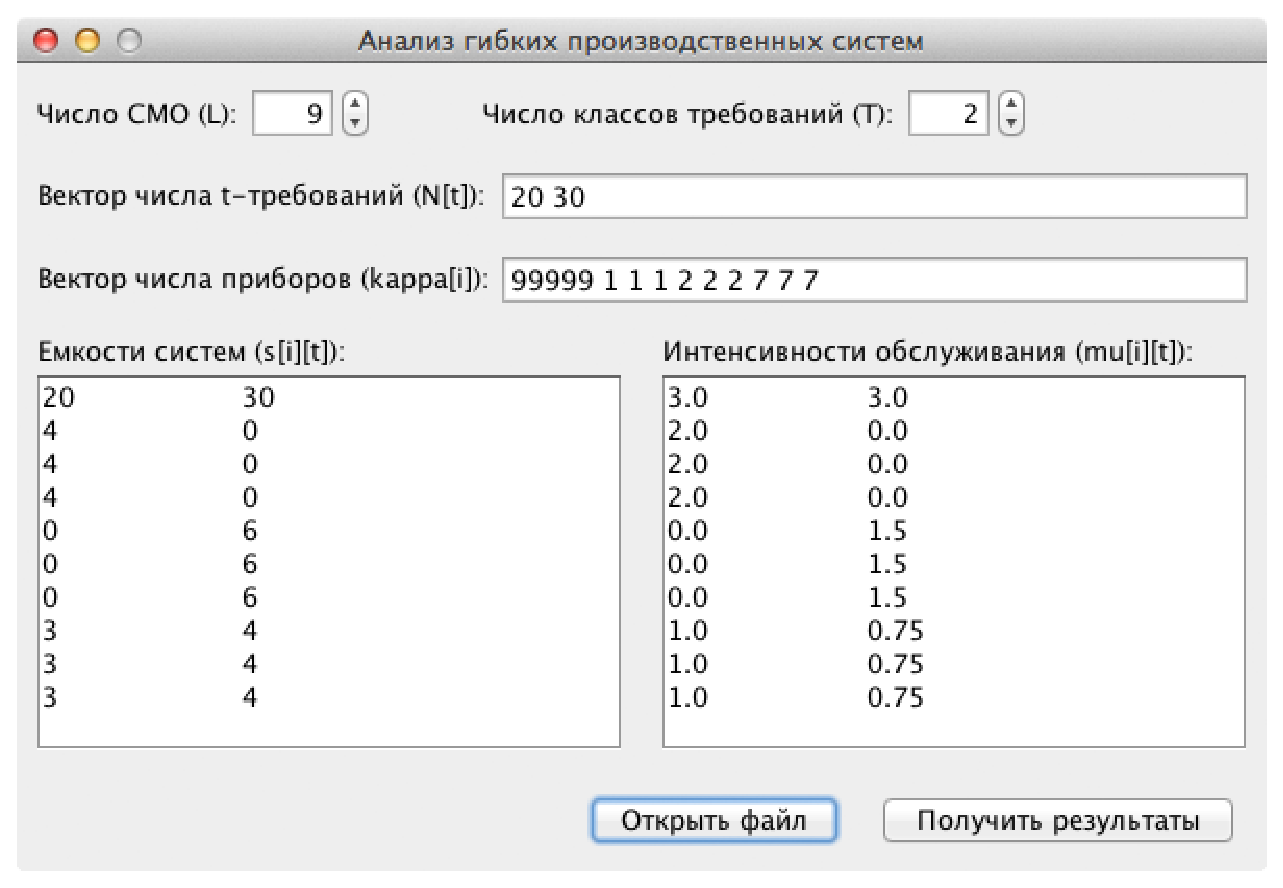
\includegraphics[width=0.9\textwidth]{main}
  \caption{}
  \label{fig:main}
\end{figure}

Для удобства существует возможность открыть файл с заданными в нем входными данными (см. рисунок \ref{fig:input}).
\begin{figure}[H]
  \centering
  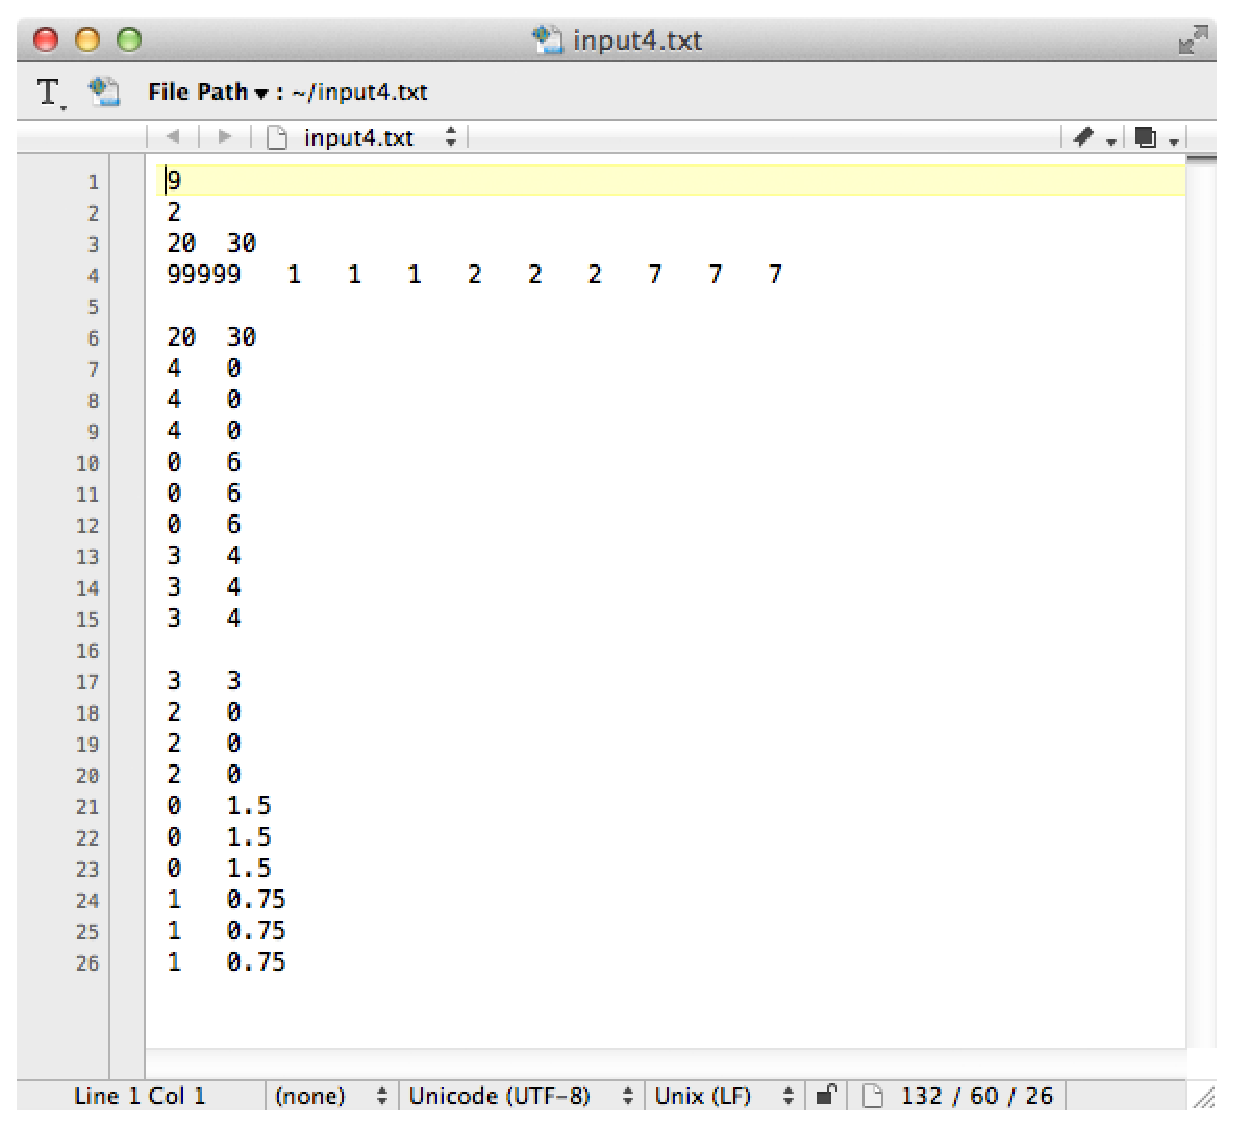
\includegraphics[width=0.9\textwidth]{input}
  \caption{}
  \label{fig:input}
\end{figure}

Для анализа при заданных входных данных служит кнопка <<Получить результаты>>. При ее нажатии открывается окно с подсчитанными в ходе анализа основными характеристиками СМО и стационарным распределением (см. рисунок \ref{fig:results}).
\begin{figure}[H]
  \centering
  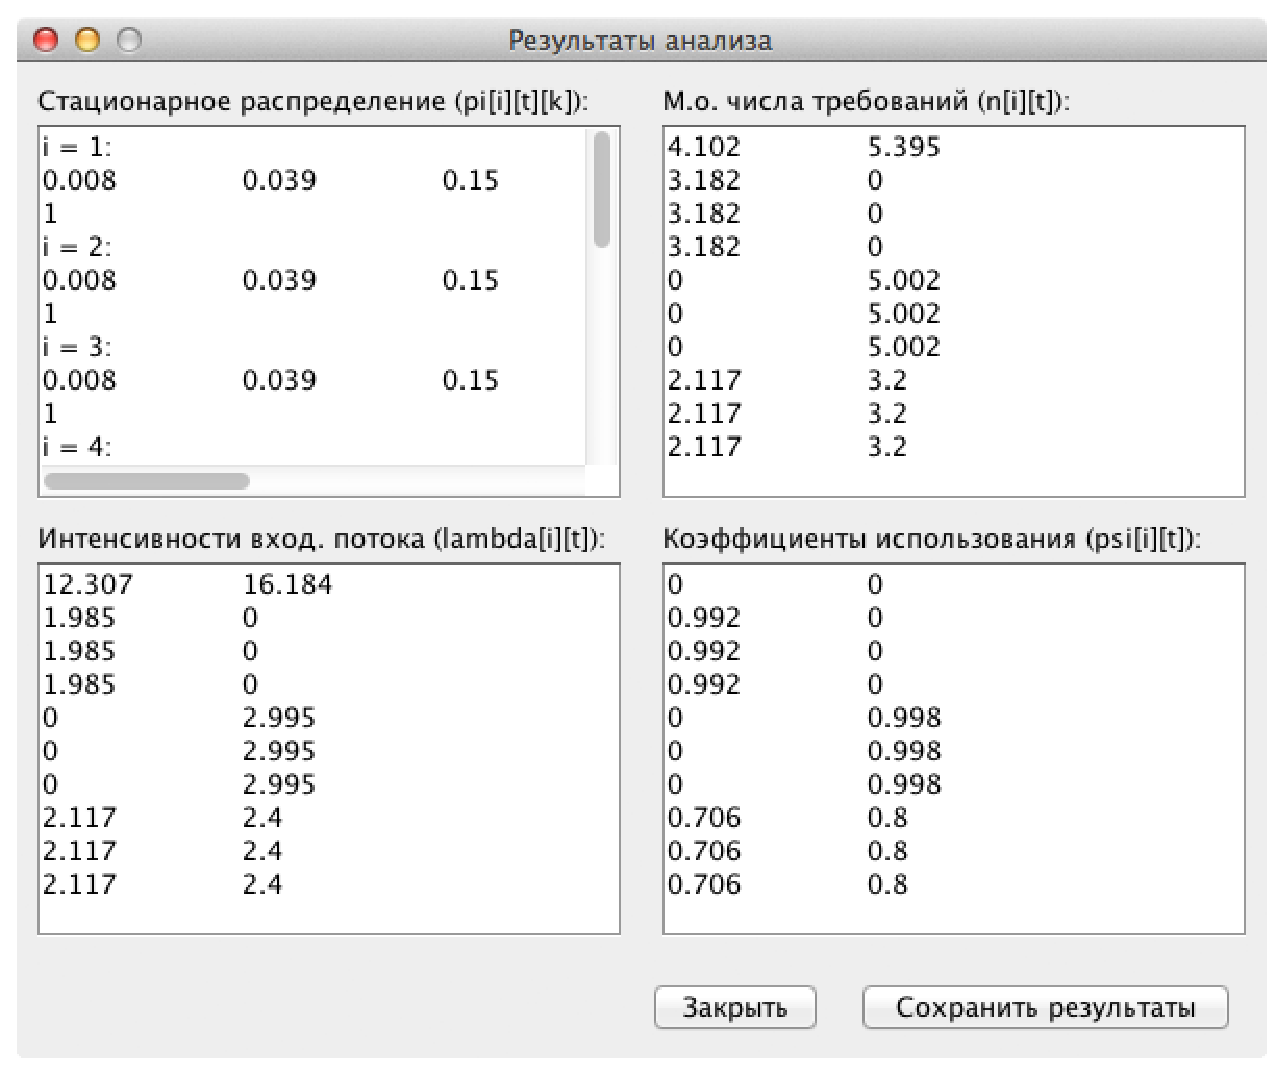
\includegraphics[width=0.9\textwidth]{results}
  \caption{}
  \label{fig:results}
\end{figure}

В случае введения некорректных начальных данных, на экран будет выведено сообщение об ошибке (см. рисунок \ref{fig:error}).
\begin{figure}[H]
  \centering
  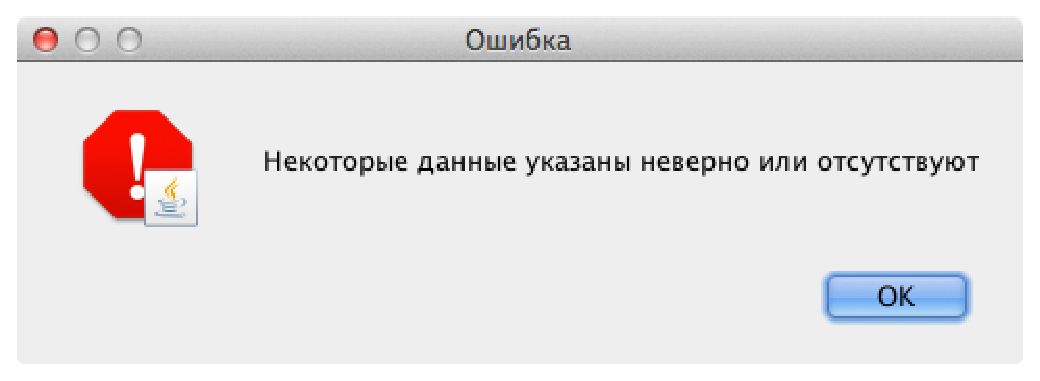
\includegraphics[width=0.75\textwidth]{error}
  \caption{}
  \label{fig:error}
\end{figure}

В окне результатов анализа пользователю предлагается на выбор два действия: закрыть окно или сохранить результаты в файл. Характеристики будут сохранены в указанный файл. На рисунке \ref{fig:output} изображен файл с результатами анализа для вышеприведенного примера (показаны не полностью):
\begin{figure}[H]
  \centering
  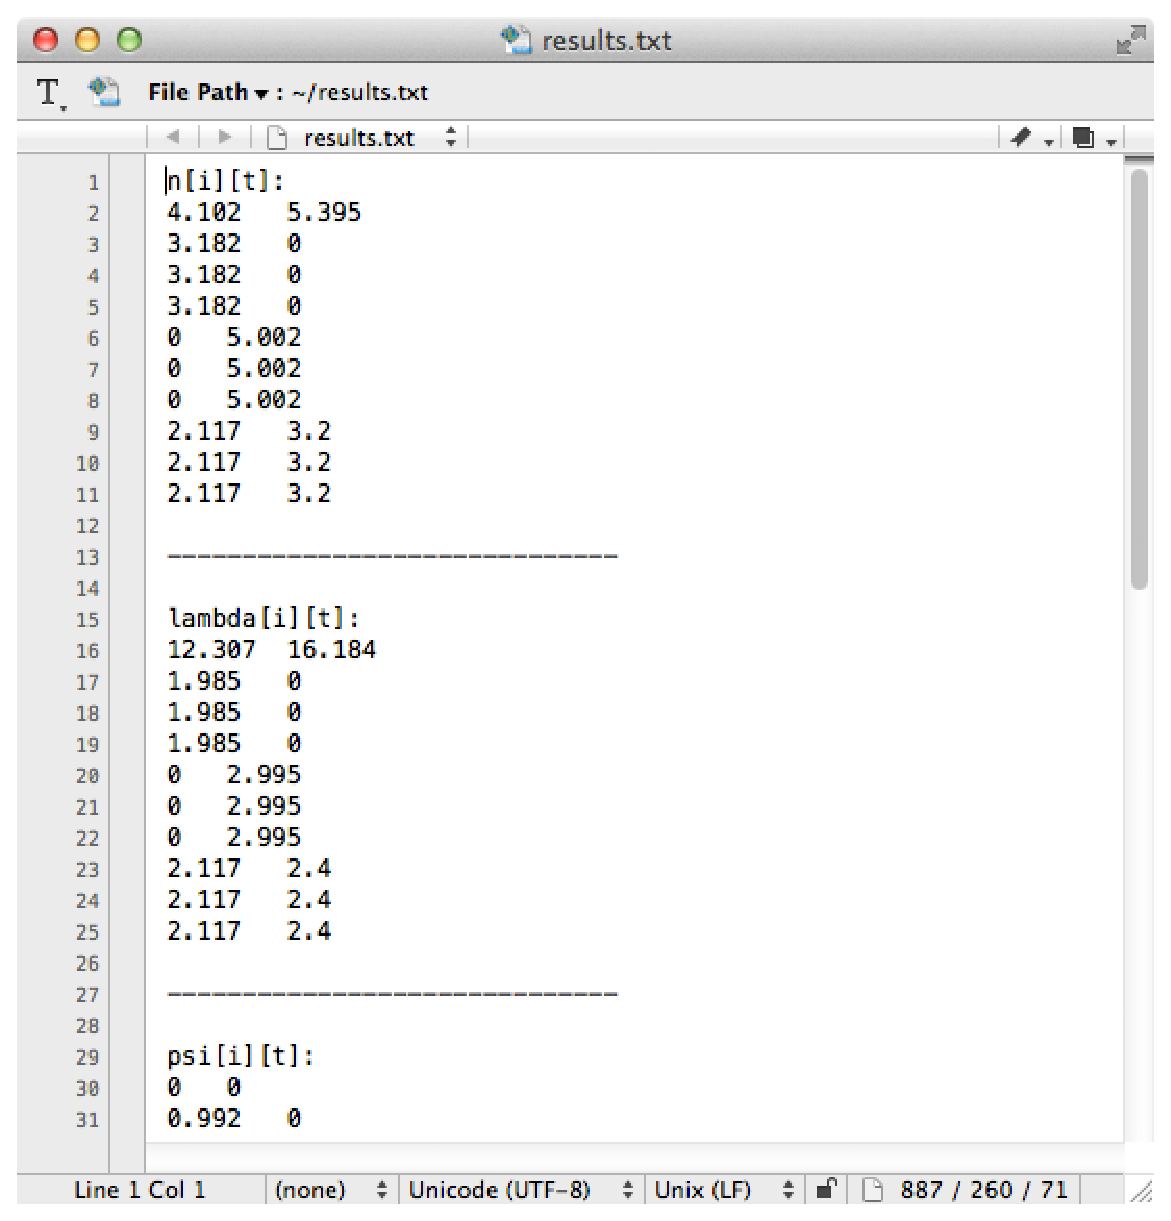
\includegraphics[width=0.9\textwidth]{output}
  \caption{}
  \label{fig:output}
\end{figure}


\subsection{Описание и назначение функций}
\label{subsec:function_description}

Функция \textit{AnalysisQueueingNetwork} является конструктором, инициализирующим  переменные класса (входные данные). Функция имеет следующую сигнатуру:
\begin{lstlisting}
public AnalysisQueueingNetwork(int L, int T, int[] N, int[] kappa, int[][] s, double[][] mu);
\end{lstlisting}
Описание параметров функции представлено в таблице \ref{tab:desc1}.

{\renewcommand{\arraystretch}{1.5}%
\begin{table}[H]
\caption{} \label{tab:desc1}
\begin{tabular}{|c|c|>{\raggedright}p{8cm}|}
	\hline
	  Параметр & Тип  & \centering{Содержание} \cr
	\hline
	  $L$ & int & Число СМО в сети \cr
	\hline
	  $T$ & int & Число классов требований в СеМО \cr
	\hline
	  $N$ & int[] & Вектор числа $t$-требований в сети \cr
	\hline
	  \textit{kappa} & int[] & Вектор числа обслуживающих приборов в СМО \cr
	\hline
	  $s$ & int[][] & Матрица емкостей систем \cr
	\hline
	  \textit{mu} & double[][] & Матрица интенсивностей обслуживания \cr
	\hline
\end{tabular}
\end{table}}

Функция \textit{analyze} является управляющей процедурой, с нее начинается анализ. Процедура для каждой системы $C_i$, $i=1,...,L$, вызывает функции \textit{swapServers} и \textit{getStateDistribution}, а затем \textit{estimateCharacteristics}. Функция имеет следующую сигнатуру:
\begin{lstlisting}
public void analyze();
\end{lstlisting}

Функция \textit{isInputDataValid} служит для проверки корректности входных данных, в частности, проверяются предположения, принятые в разделе \ref{subsec:FMS_specification}. Функция имеет следующую сигнатуру:
\begin{lstlisting}
public static boolean isInputDataValid(int L, int T, int[] N, int[] kappa, int[][] s, double[][] mu);
\end{lstlisting}
Параметры функции были описаны выше. Функция возвращает true, если данные корректны, и false в противном случае.

Функция \textit{swapServers} для анализа текущей системы переставляет ее с последней системой сети путем перестановки соответствующих индексов входных данных. Функция имеет следующую сигнатуру:
\begin{lstlisting}
private void swapServers(int i);
\end{lstlisting}
Описание параметров функции представлено в таблице \ref{tab:desc2}.

{\renewcommand{\arraystretch}{1.5}%
\begin{table}[H]
\caption{} \label{tab:desc2}
\begin{tabular}{|c|c|>{\raggedright}p{4cm}|}
	\hline
	  Параметр & Тип & \centering{Содержание} \cr
	\hline
	  $i$ & int & Номер СМО $C_i$ \cr
	\hline
\end{tabular}
\end{table}}

Функция \textit{getStateDistribution} вычисляет стационарное распределение вероятностей состояний для текущей системы. Функция имеет следующую сигнатуру:
\begin{lstlisting}
private double[][] getStateDistribution();
\end{lstlisting}
Описание вычисляемых функцией данных представлено в таблице \ref{tab:desc3}.

{\renewcommand{\arraystretch}{1.5}%
\begin{table}[H]
\caption{} \label{tab:desc3}
\begin{tabular}{|c|c|>{\raggedright}p{7cm}|}
	\hline
	Имя переменной & Тип  & \centering{Содержание} \cr
	\hline
	  $pi$ & double[][] &  Стационарное распределение вероятностей состояний для системы $C_i$ \cr
	\hline
\end{tabular}
\end{table}}

Функция \textit{f} вычисляет множитель в выражении (\ref{eq:2.4}). Функция имеет следующую сигнатуру:
\begin{lstlisting}
private double f(int i, int t, int n);
\end{lstlisting}
Описание параметров функции представлено в таблице \ref{tab:desc4}.

{\renewcommand{\arraystretch}{1.5}%
\begin{table}[H]
\caption{} \label{tab:desc4}
\begin{tabular}{|c|c|>{\raggedright}p{7cm}|}
	\hline
	  Параметр & Тип  & \centering{Содержание} \cr
	\hline
	  $i$ & int & Номер СМО $C_i$ \cr
	\hline
	  $t$ & int & Номер класса требований \cr
	\hline
	  $n$ & int & Число $t$-требований в системе $i$ \cr
	\hline
\end{tabular}
\end{table}}


Функция \textit{estimateCharacteristics} вычисляет стационарные характеристики сети, а именно м. о. числа $t$-требований в СМО $C_i$, интенсивности потока $t$-требований в $C_i$ и коэффициенты использования обслуживающих приборов системы $C_i$ $t$-требованиями, $i=1,...,L$. Также дополнительно происходит вычисление вышеперечисленных характеристик для $C_0$, которая представляет собой систему транспортировки в ГПС. Функция имеет следующую сигнатуру:
\begin{lstlisting}
private void estimateCharacteristics();
\end{lstlisting}
Описание вычисляемых функцией данных представлено в таблице \ref{tab:desc5}.

{\renewcommand{\arraystretch}{1.5}%
\begin{table}[H]
\caption{} \label{tab:desc5}
\begin{tabular}{|c|c|>{\raggedright}p{7cm}|}
	\hline
	  Имя переменной & Тип  & \centering{Содержание} \cr
	\hline
	  $charN$ & double[][] &  М. о. числа $t$-требований в СМО $C_i$ \cr
	\hline
	  $charLambda$ & double[][] & Интенсивности потока $t$-требований в $C_i$ \cr
	\hline
	  $charPsi$ & double[][] & Коэффициенты использования обслуживающих приборов системы $C_i$ $t$-требованиями \cr
	\hline
\end{tabular}
\end{table}}


%%%%%%%%%%%%%%%%%%%%%%%%%%%%%%%%%%%%%%%%%%%%%%%%%%%%%%%%%%%%%%%%%%%%%%%%%%%%%%%


\section{Аспекты практического применения}
\label{sec:practical_application}

Было проведено несколько серий экспериментов с использованием разработанной программы анализа производственных систем с маршрутизацией, зависящей от состояния.

\textbf{Эксперимент 1}

Рассмотрим гибкую производственную систему с двумя рабочими станциями ($C_1$ и $C_2$), каждая из которых имеет два параллельных прибора \cite{yao1}.  Две рабочие станции связаны друг с другом циклическим конвейером $C_0$, где каждая деталь имеет единичную среднюю задержку (время в пути), т.е. $\mu_0=1$. Пусть $N=8$ (общее количество деталей в системе), а $s_1=s_2=4$ (т.е. существует 2 лишних места в очереди каждой станции). Также предположим, что длительности обработки на обеих станциях имеют экспоненциальное распределение, причем средняя длительность обработки на обеих станциях равна $1,9$.

Используя алгоритм анализа производственных систем с PSQ-маршрутизацией, получим результаты, приведенные в таблице \ref{tab:result1}.

{\renewcommand{\arraystretch}{1.5}%
\begin{table}[H]
\caption{} \label{tab:result1}
\begin{tabular}{|c|c|c|}
	\hline
	$C_i$ &  $C_0$  & $C_{1, 2}$  \cr
	\hline
	$\overline{n}_i$  &  2,014  &  2,993  \cr
	\hline
	$\lambda_i$  &  2,014  &  1.007  \cr
	\hline
	$\psi_i$  &  --   &  0,957  \cr
	\hline
\end{tabular}
\end{table}}

\textbf{Эксперимент 2}

Рассмотрим гибкую производственную систему с 14 машинами, сгруппированными по 7 рабочим станциям. Число приборов, интенсивность обработки детали одним прибором и емкость локального хранилища на каждой станции соответственно равны: \\
$\kappa_1=\kappa_2=1$; $\kappa_3=\kappa_4=\kappa_5=2$; $\kappa_6=\kappa_7=3$; \\
$\mu_1=\mu_2=3$; $\mu_3=\mu_4=\mu_5=1,5$; $\mu_6=\mu_7=1$; \\
$s_1=s_2=5$; $s_3=s_4=s_5=6$; $s_6=s_7=7$. \\
Число транспортеров $\kappa_0=7$, каждый из которых имеет интенсивность обработки $\mu_0=4$. В данной системе есть $N=30$ палет, т.е. общее число деталей (одного типа) в любой момент времени равно $30$.

В таблице \ref{tab:result2} приведены основные характеристики гибкой производственной системы c PSQ--маршрутизацией.

{\renewcommand{\arraystretch}{1.5}%
\begin{table}[H]
\caption{} \label{tab:result2}
\begin{tabular}{|c|c|c|c|c|}
	\hline
	$C_i$ & $C_0$ & $C_{1, 2}$ & $C_{3, 4, 5}$ & $C_{6, 7}$ \cr
	\hline
	$\overline{n}_i$  &  5,511  &  2,549  &  3,491  &  4,460 \cr
	\hline
	$\lambda_i$  &  19,804  &  2,768  &  2,839  &  2,875 \cr
	\hline
	$\psi_i$  &    0,707  &  0,923  &  0,946  &  0,958 \cr
	\hline
\end{tabular}
\end{table}}

\textbf{Эксперимент 3}

Сравним PSQ--маршрутизацию с DSQ--маршрутизацией. Рассмотрим производственную систему с $18$ машинами, которые сгруппированы по $9$ рабочим станциям. Число приборов, интенсивность обработки детали одним прибором и емкость локального хранилища на каждой станции соответственно равны: \\
$\kappa_1=\kappa_2=\kappa_3=1$; $\kappa_4=\kappa_5=\kappa_6=2$; $\kappa_7=\kappa_8=\kappa_9=3$; \\
$\mu_1=\mu_2=\mu_3=2$; $\mu_4=\mu_5=\mu_6=1,5$; $\mu_7=\mu_8=\mu_9=1$; \\
$s_1=s_2=s_3=4$; $s_4=s_5=s_6=6$; $s_7=s_8=s_9=7$. \\
Число транспортеров $\kappa_0=9$, каждый из которых имеет интенсивность обработки $\mu_0=3$. В данной системе есть $N=50$ палет, т.е. общее число деталей (одного типа) в любой момент времени равно $50$. Мы сравним производительность производственной системы, имеющей PSQ--маршрутизацию, с производственной системой, имеющей DSQ--маршрутизацию, где вероятность перехода от станции $C_0$ к станциям $C_1$, $C_2$ и $C_3$ равна $2/24$, а к другим станциям~--- $3/24$. 

Математическое ожидание числа деталей ($\overline{n}_i$), пропускная способность ($\lambda_i$) и коэффициенты использования приборов ($\psi_i$) для каждой станции приведены в таблице~\ref{tab:result3} (в скобках указаны результаты для DSQ--маршрутизации). PSQ--маршрутизация имеет очевидные преимущества с точки зрения увеличения пропускной способности, а также коэффициентов использования приборов и очередей производственной системы \cite{yao1}.

{\renewcommand{\arraystretch}{1.5}%
\begin{table}[H]
\caption{} \label{tab:result3}
\begin{tabular}{|c|c|c|c|c|}
\hline
$C_i$ & $C_0$ & $C_{1, 2, 3}$ & $C_{4, 5, 6}$ & $C_{7, 8, 9}$ \cr
\hline
$\overline{n}_i$  &  11,070 (18,937)  &  3,003 (2,230)  &  4,492 (3,638)  &  5,482 (4,486) \cr
\hline
$\lambda_i$  &  23,595 (21,168)  &  1,954 (1,687)  &  2,950 (2,672)  &  2,961 (2,697) \cr
\hline
$\psi_i$  &  0,874 (0,784)  &  0,977 (0,844)  &  0,983 (0,891)  &  0,987 (0,899) \cr
\hline
\end{tabular}
\end{table}}

\textbf{Эксперимент 4}

Теперь изменим вышеприведенный пример следующим образом: в системе имеется два типа деталей и $50$ палет разделяются на $N_1=20$ и $N_2=30$. Первый тип деталей посещает только станции $C_1$, $C_2$, $C_3$ и $C_7$, $C_8$, $C_9$, а второй тип~--- только станции $C_4$, $C_5$, $C_6$ и $C_7$, $C_8$, $C_9$. Станции $C_7$, $C_8$ и $C_9$ имеют по $7$ приборов без дополнительного ожидания. На каждой из этих трех станций первый тип деталей может занимать до 3 приборов и интенсивность обработки деталей $\mu_{i1}=1$ ($i=7,8,9$), второй тип может занимать до 4 приборов и интенсивность обработки деталей $\mu_{i2}=0,75$ ($i=7,8,9$). Система транспортировки материалов представляет собой циклический конвейер, моделируемый как система с бесконечным числом приборов (то есть все требования обслуживаются сразу после поступления в систему), где среднее время пребывания каждого класса требований $\mu_0^{-1}=1/3$ \cite{yao1}.

То есть мы имеем следующие данные: \\
$L=9$; $T=2$; $\mathbf{N}=(20,30)$; \\
$I_1=\{1,2,3,7,8,9\}$, $I_2=\{4,5,6,7,8,9\}$; \\
$\kappa_1=\kappa_2=\kappa_3=1$; $\kappa_4=\kappa_5=\kappa_6=2$; $\kappa_7=\kappa_8=\kappa_9=7$; \\
$\mu_{11}=\mu_{21}=\mu_{31}=2$; $\mu_{42}=\mu_{52}=\mu_{62}=1,5$; $\mu_{71}=\mu_{81}=\mu_{91}=1$; $\mu_{72}=\mu_{82}=\mu_{92}=0,75$; \\
$s_{11}=s_{21}=s_{31}=4$; $s_{42}=s_{52}=s_{62}=6$; $s_{71}=s_{81}=s_{91}=3$; $s_{72}=s_{82}=s_{92}=4$. \\
Для $C_0$: $\mu_{01}=\mu_{02}=3$; $s_{01}=20$; $s_{02}=30$. \\

В таблице \ref{tab:result4} приводятся соответствующие результаты анализа.

{\renewcommand{\arraystretch}{1.5}%
\begin{table}[H]
\caption{} \label{tab:result4}
\begin{tabular}{|c|c|c|c|c|c|c|}
\hline
$C_i$  &  \multicolumn{2}{c|}{$C_0$}  &  $C_{1, 2, 3}$  &  $C_{4, 5, 6}$  &  \multicolumn{2}{c|}{$C_{7, 8, 9}$} \cr
\hline
$t$ &  Тип 1  &  Тип 2  &  Тип 1  &  Тип 2  &  Тип 1  &  Тип 2 \cr
\hline
$\overline{n}_i$  &  4,102  &  5,395  &  3,182  &  5,002  &  2,117  &  3,200 \cr
\hline
$\lambda_i$  & 12,307  & 16,184  &  1,985  &  2,995  &  2,117  &  2,400 \cr
\hline
$\psi_i$  &    --    &    --    &  0,993  &  0,998  &  0,706  &  0,800 \cr
\hline
\end{tabular}
\end{table}}

\textbf{Эксперимент 5}

Возьмем гибкую производственную систему из примера 3 и посмотрим, как будут изменяться характеристики рабочих станций $C_i$, $i=1,2$, с изменением числа приборов, емкостей рабочих станций и интенсивностей обработки деталей (эти данные предполагаются одинаковыми для обеих рабочих станций). Результаты представлены на рисунках \ref{fig:graph1}--\ref{fig:graph3}.

\begin{figure}[H]
  \centering
  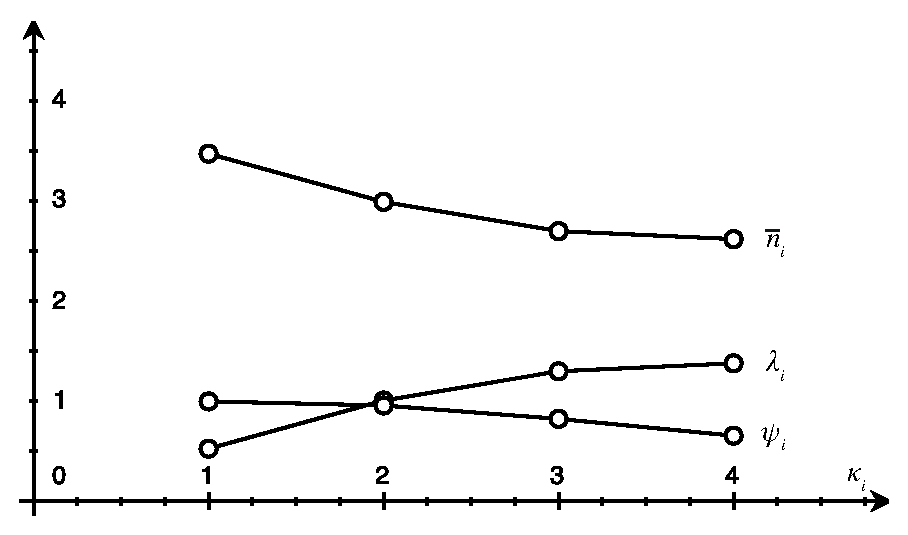
\includegraphics[]{graph1}
  \caption{Зависимость стационарных характеристик ГПС от числа приборов}
  \label{fig:graph1}
\end{figure}

\begin{figure}[H]
  \centering
  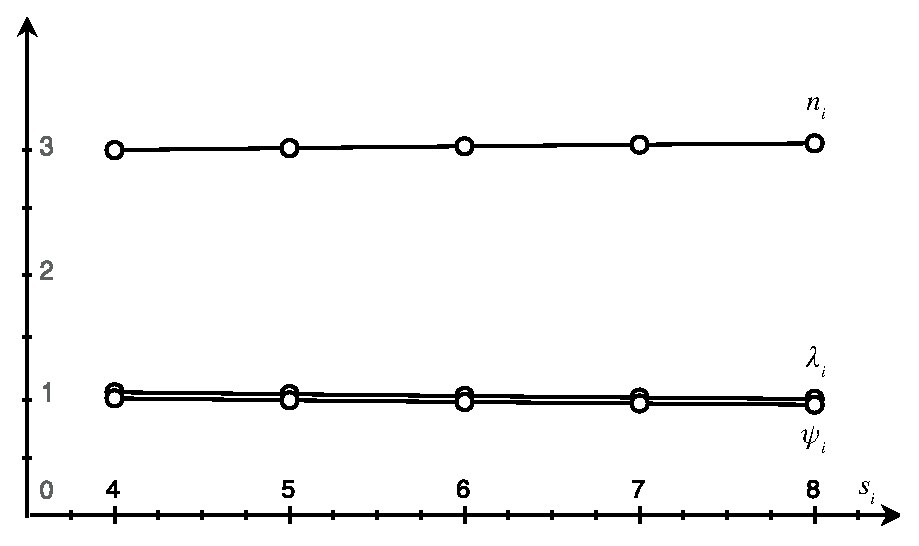
\includegraphics[]{graph2}
  \caption{Зависимость стационарных характеристик ГПС от емкостей рабочих станций}
  \label{fig:graph2}
\end{figure}

\begin{figure}[H]
  \centering
  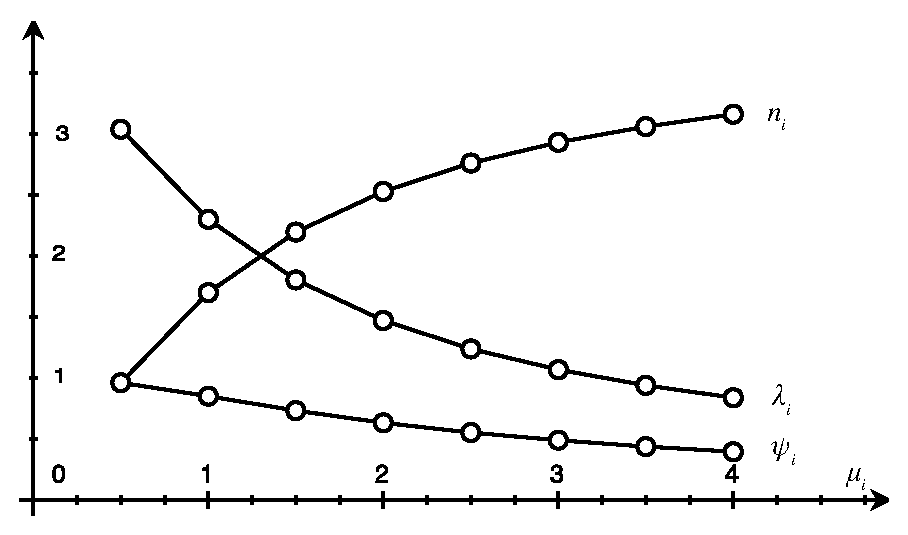
\includegraphics[]{graph3}
  \caption{Зависимость стационарных характеристик ГПС от интенсивностей обработки деталей}
  \label{fig:graph3}
\end{figure}

Помимо характеристик гибкой производственной системы, программа генерирует все распределения вероятностей. Время выполнения этих примеров на современном персональном компьютере~--- доли секунды.


%%%%%%%%%%%%%%%%%%%%%%%%%%%%%%%%%%%%%%%%%%%%%%%%%%%%%%%%%%%%%%%%%%%%%%%%%%%%%%%


\conclusion
Основной целью выпускной квалификационной работы являлось исследование производственных систем с маршрутизацией, зависящей от состояния, разработка алгоритма метода анализа данных производственных систем, программная реализация алгоритма. Результатами работы являются следующие:

\begin{itemize}
\item рассмотрены производственные системы с маршрутизацией, зависящей от состояния;
\item приведено доказательство того, что при PSQ--маршрутизации марковский процесс обратим относительно времени и имеет мультипликативную форму стационарного распределения;
\item разработан алгоритм метода анализа производственных систем с маршрутизацией, зависящей от состояния;
\item разработана программа, вычисляющая основные стационарные характеристики;
\item проведены численные эксперименты с разработанной программой и приведены соответствующие результаты.
\end{itemize}

Эта модель может быть использована при решении задач анализа и оптимизации гибких производственных систем.



% Список использованных источников
\begin{thebibliography}{9}

\bibitem{mitrofanov}
 Митрофанов Ю. И. Анализ сетей массового обслуживания.~-- Саратов: Научная книга, 2005.~-- 175 с.

\bibitem{kleinrock1}
 Клейнрок Л. Теория массового обслуживания / Пер. с англ.~-- М.: Машиностроение, 1979.~-- 432 с.

\bibitem{kleinrock2}
 Клейнрок Л. Вычислительные системы с очередями / Пер. с англ.~-- М.: Мир, 1979.~-- 600 с.

\bibitem{gnedenko}
 Гнеденко Б. В., Коваленко И. Н. Введение в теорию массового обслуживания.~-- М.: Наука, ГРФМЛ, 1966.~-- 432 c.

\bibitem{yao1}
 Yao D. D., Buzacott J. A. Modeling a class of state-dependent routing in flexible manufacturing systems~// Annals of Operations Research.~-- 1985.~-- No. 3.~-- P. 153-167.

\bibitem{yao2}
 Yao D. D., Buzacott J. A. On queueing network as flexible manufacturing systems~// Queueing Systems.~--1986.~-- No 1.~-- P. 5-27.

\bibitem{yao3}
 Yao D. D., and Buzacott J. A. Modeling the performance of flexible manufacturing systems~// International Journal of Production Research.~--1984.~-- Vol. 23.~-- P. 945-955.

\bibitem{reiser}
 Reiser M., Lavenberg S. S. Mean-value analysis of closed multichain queueing networks~// J. of the Association for Computing Machinery.~-- 1980.~-- Vol. 27, No. 2.~-- P. 313-322.

\bibitem{kelly}
 Kelly F. P. Reversibility and stochastic networks.~-- New York: Wiley, 1979.

\end{thebibliography}



% Приложения
\appendix

\section{Код программы} \label{appendix:A}

\lstinputlisting{sources/AnalysisFMS.java}
\clearpage
\lstinputlisting{sources/AnalysisQueueingNetwork.java}
\clearpage
\lstinputlisting{sources/ResultFrame.java}

\end{document}
